\subsection{可积函数的 Fourier 变换}

本节回顾 Spectral Theories\(^{6}\) 中的一些定义和结果。

记 \(\hat{\mathbf{G}}\) 为 \(\mathbf{G}\) 的不可约表示（作用在有限维复向量空间上）的等价类集合。对于所有 \(u\in \hat{\mathbf{G}}\)，记 \(\mathrm{E}_u\) 为 \(u\) 的表示空间，记 \(d(u)\) 为其维数。\(\mathrm{E}_u\) 上存在在 \(u\) 下不变的分离的正埃尔米特型，且任意两个这样的型成比例。相对于这些型中的一个，记 \(\mathrm{A}^*\)（相应地，\(\| \mathrm{A}\|_{\infty}\)）为元素 \(\mathrm{A}\) 在 \(\operatorname {End}(\mathrm{E}_u)\) 中的伴随（相应地，其范数）；对于所有 \(g\in \mathbf{G}\)，有 \(u(g)^{*} = u(g)^{-1} = u(g^{-1})\) 且 \(\| u(g)\|_{\infty} = 1\)；对于所有 \(x\in \mathfrak{g}\)，有 \(u(x)^{*} = -u(x) = u(-x)\)。

在 \(\operatorname{End}(\mathbf{E}_u)\) 上赋予希尔伯特空间结构，使其内积为

\[
\langle \mathrm{A} | \mathrm{B} \rangle = d (u) \mathrm{Tr} (\mathrm{A} ^ {*} \mathrm{B}) = d (u) \mathrm{Tr} (\mathrm{BA} ^ {*}),\tag{1}
\]

并令

\[
\| \mathrm{A} \| _ {2} = \langle \mathrm{A} | \mathrm{A} \rangle^ {1 / 2} = (d (u) \mathrm{Tr} (\mathrm{A} ^ {*} \mathrm{A})) ^ {1 / 2}.\tag{2}
\]

有

\[
\sqrt {d (u)} \| \mathrm{A} \| _ {\infty} \leq \| \mathrm{A} \| _ {2} \leq d (u) \| \mathrm{A} \| _ {\infty},\tag{3}
\]

因此

\[
| \langle \mathrm{A} | \mathrm{B} \rangle | \leq d (u) ^ {2} \| \mathrm{A} \| _ {\infty} \| \mathrm{B} \| _ {\infty}.\tag{4}
\]

对于所有 \(g \in \mathrm{G}\)，有 \(\| u(g) \|_2 = d(u)\)。

记 \(\mathrm{F}(\hat{\mathrm{G}})\) 为代数 \(\prod_{u\in \hat{\mathrm{G}}}\mathrm{End}(\mathrm{E}_u)\)。记 \(\mathrm{L}^2 (\hat{\mathrm{G}})\) 为希尔伯特空间 \(\mathrm{End}(\mathrm{E}_u)\) 的希尔伯特和；它是由族 \(\mathrm{A} = (\mathrm{A}_u)\in \mathrm{F}(\hat{\mathrm{G}})\) 构成的空间，其中满足 \(\sum_{u}\| \mathrm{A}_{u}\|_{2}^{2} < \infty\)，其内积为

\[
\langle \mathrm{A} | \mathrm{B} \rangle = \sum_ {u \in \hat {\mathrm{G}}} \langle \mathrm{A} _ {u} | \mathrm{B} _ {u} \rangle = \sum_ {u \in \hat {\mathrm{G}}} d (u) \operatorname{Tr} (\mathrm{A} _ {u} ^ {*} \mathrm{B} _ {u}).\tag{5}
\]

\(L^{2}(\hat{G})\) 上的希尔伯特范数也记作 \(\parallel\parallel_{2}\)，于是有 \(\|A\|_{2}^{2}=\sum_{u\in\hat{G}}\|A_{u}\|_{2}^{2}\)，其中 \(A\in L^{2}(\hat{G})\)。

若 \(f\) 是 \(G\) 上的可积复函数，定义

\[
u (f) = \int_ {\mathrm{G}} f (g) u (g) d g \in \operatorname{End} (\mathrm{E} _ {u})\tag{6}
\]

对于所有 \(u \in \hat{\mathbf{G}}\)。有 \(\| u(f) \|_{\infty} \leq \int_{\mathbf{G}} |f(g)| dg = \| f \|_1\)。\(f\) 的 Fourier 余变换记为 \(\overline{\mathcal{F}}(f)\)，它是族 \((u(f))_{u \in \hat{\mathbf{G}}} \in \mathrm{F}(\hat{\mathbf{G}})\)。若 \(f \in \mathrm{L}^2(\hat{\mathbf{G}})\)，

\[
\| f \| _ {2} ^ {2} = \sum_ {u \in \hat {\mathsf {G}}} \langle u (f) | u (f) \rangle = \| \overline {{\mathcal {F}}} (f) \| _ {2} ^ {2},
\]

因此 \(\overline{F}\) 诱导出从希尔伯特空间 \(\mathrm{L}^{2}(\mathrm{G})\) 到希尔伯特空间 \(\mathrm{L}^{2}(\hat{\mathrm{G}})\) 的等距线性映射；换言之，对于 f 和 \(f'\) 属于 \(\mathrm{L}^{2}(\mathrm{G})\)，有

\[
\int_ {\mathrm{G}} \overline {{f (g)}} f ^ {\prime} (g) d g = \langle \overline {{\mathcal {F}}} (f) | \overline {{\mathcal {F}}} (f ^ {\prime}) \rangle = \sum_ {u \in \hat {\mathrm{G}}} d (u) \mathrm{Tr} (u (f) ^ {*} u (f ^ {\prime})).\tag{7}
\]

对于 \(f\) 和 \(f'\) 属于 \(\mathrm{L}^1(\mathrm{G})\)，\(f * f'\) 是 \(f\) 与 \(f'\) 的卷积积，定义为

\[
(f * f ^ {\prime}) (h) = \int_ {G} f (h g ^ {- 1}) f ^ {\prime} (g) d g = \int_ {G} f (g) f ^ {\prime} (g ^ {- 1} h) d g
\]

（该积分对几乎所有 \(h \in \mathbf{G}\) 都有意义）。

有 \(f * f' \in L^{1}(G)\)，且对于所有 \(u \in \hat{G}\)，\(u(f * f') = u(f)u(f')\)，故

\[
\overline {{{{\mathcal {F}}}}} (f * f ^ {\prime}) = \overline {{{{\mathcal {F}}}}} (f). \overline {{{{\mathcal {F}}}}} (f ^ {\prime}).\tag{8}
\]

反之，设 \(\mathrm{A} = (\mathrm{A}_{u})_{u \in \hat{\mathrm{G}}}\) 是 \(\mathrm{F}(\hat{\mathrm{G}})\) 的一个元素；对于所有 \(u \in \hat{G}\)，令 \(F_{u}A\) 为 G 上由下式定义的（解析）函数

\[
(\mathcal {F} _ {u} \mathrm{A}) (g) = \langle u (g) | \mathrm{A} _ {u} \rangle = d (u) \mathrm{Tr} (\mathrm{A} _ {u} u (g) ^ {- 1}).\tag{9}
\]

若 \(\mathrm{A} \in \mathrm{L}^2(\hat{\mathrm{G}})\)，族 \((\mathcal{F}_u\mathrm{A})_{u \in \hat{\mathrm{G}}}\) 在 \(\mathrm{L}^2(\mathrm{G})\) 中可求和；\(\mathrm{A}\) 的 Fourier 变换记为 \(\mathcal{F}(\mathrm{A})\)，定义为该族之和。映射 \(\overline{\mathcal{F}}\) 和 \(\mathcal{F}\) 是希尔伯特空间 \(\mathrm{L}^2(\mathrm{G})\) 与 \(\mathrm{L}^2(\hat{\mathrm{G}})\) 之间的互逆同构。

换言之：

命题 1. 每个平方可积复函数 \(f\)（定义在 \(G\) 上）都是在希尔伯特空间 \(L^2(G)\) 中族 \((f_u)_{u\in \hat{G}}\) 的和，其中对于所有 \(h\in G\) 和所有 \(u\in \hat{G}\)，

\[
\begin{array}{l} f _ {u} (h) = \langle u (h) | u (f) \rangle \\ \qquad = d (u) \int_ {\mathrm{G}} f (g) \mathrm{Tr} (u (g h ^ {- 1}))   d g = d (u) \int_ {\mathrm{G}} f (g h) \mathrm{Tr} (u (g))   d g. \end{array}\tag{10}
\]

对于所有 \(u \in \hat{\mathrm{G}}\)，选取 \(\mathrm{B}_u\) 作为 \(\mathrm{E}_u\) 的一个规范正交基，并记 \((u_{ij}(g))\) 为此基下 \(u(g)\) 的矩阵。命题 1 还意味着，函数族 \(\sqrt{d(u)} u_{ij}\)（其中 \(u\) 属于 \(\hat{\mathrm{G}}\) 且 \(i,j\) 属于 \(\mathrm{B}_u\)）是空间 \(\mathrm{L}^2 (\mathrm{G})\) 的一个规范正交基。

若 f 是 G 上的可积函数且族 \((f_{u})\) 一致可求和，则该族之和是一个几乎处处与 f 一致的连续函数；换言之，若再假定 f 连续，则对于所有 \(h \in G\)，

\[
f (h) = \sum_ {u \in \hat {\mathrm{G}}} d (u) \int_ {\mathrm{G}} f (g h) \mathrm{Tr} (u (g))   d g.\tag{11}
\]

反之，设 \(\mathrm{A} \in \mathrm{F}(\hat{\mathrm{G}})\)；若族 \((\mathcal{F}_u\mathrm{A})_{u \in \hat{\mathrm{G}}}\) 一致可求和，则函数

\[
g \mapsto \sum_ {u \in \hat {\mathrm{G}}} (\mathcal {F} _ {u} \mathrm{A}) (g) = \sum_ {u \in \hat {\mathrm{G}}} d (u) \mathrm{Tr} (\mathrm{A} _ {u} u (g) ^ {- 1})
\]

是 \(G\) 上的连续函数，其 Fourier 余变换为 \(A\)。

设 \(f\) 是 \(\mathbf{G}\) 上的可积函数，且 \(s \in \mathbf{G}\)。记 \(\gamma(s)f\) 和 \(\delta(s)f\) 为 \(\mathbf{G}\) 上由 \(\gamma(s)f = \varepsilon_s * f\)、\(\delta(s)f = f * \varepsilon_{s^{-1}}\) 定义的函数，即

\[
(\gamma (s) f) (g) = f (s ^ {- 1} g), \quad (\delta (s) f) (g) = f (g s) \text { for } g \in \mathrm{G},
\]

(Chap. III, §3, no. 4 and Integration, Chap. VII, §1, no. 1). 有

\[
u (\gamma (s) f) = \int_ {\mathrm{G}} f (s ^ {- 1} g) u (g) d g = \int_ {\mathrm{G}} f (g) u (s g) d g,
\]

因此

\[
u (\gamma (s) f) = u (s) u (f),\tag{12}
\]

类似地

\[
u (\delta (s ^ {- 1}) f) = u (f) u (s).\tag{13}
\]

当 G 交换时，\(\hat{G}\) 是 G 的对偶群的底层集合（Spectral Theories, Chap. II, §1, no. 1），且 \(d(u) = 1\) 对所有 \(u \in \hat{G}\) 成立，于是我们得到 Spectral Theories, Chap. II 中给出的 Fourier 变换定义。

\subsection{无穷次可微函数的 Fourier 变换}

回忆 (Chap. III, §3, no. 1, Def. 2)，U(G) 表示支集包含于 \(\{e\}\) 的 G 上分布所成的代数。g 到 U(G) 的典则嵌入延拓为从李代数 g 的包络代数到 U(G) 的同构 (loc. cit., no. 7, Prop. 25)；以下通过此同构识别这两个代数。若 f 是 G 上的无穷次可微复函数，且 \(t \in \mathrm{U}(\mathrm{G})\)，记 \(L_{t}f\) 和 \(R_{t}f\) 为 G 上由下式定义的函数

\[
\mathrm{L} _ {t} f (g) = \langle \varepsilon_ {g} * t, f \rangle , \quad \mathrm{R} _ {t} f (g) = \langle t * \varepsilon_ {g}, f \rangle
\]

(cf.~loc. cit., no. 6). 对于所有 \(g \in G\)，

\[
\mathrm{L} _ {t} \circ \gamma (g) = \gamma (g) \circ \mathrm{L} _ {t}, \quad \mathrm{R} _ {t} \circ \delta (g) = \delta (g) \circ \mathrm{R} _ {t}.
\]

设 \(u \in \hat{G}\)；记 \(E_u\) 为 \(u\) 的表示空间。李群态射 \(u: G \to \mathbf{GL}(E_u)\) 经微分给出实李代数的同态 \(\mathfrak{g} \to \text{End}(E_u)\)，从而给出代数同态，仍记作 \(u\)，即从 \(U(G)\) 到 \(\text{End}(E_u)\) 的同态。若 \(t \in U(G)\) 且 \(f\) 是 \(G\) 上的无穷次可微函数，则

\[
u (\mathrm{L} _ {t} f) = u (f) u (t ^ {\vee}), \quad u (\mathrm{R} _ {t} f) = u (t ^ {\vee}) u (f),\tag{14}
\]

其中 \(t^{\vee}\) 表示 t 在 U(G) 的主反自同构下的像 (Chap. I, §2, no. 4)；事实上，只需对 \(t \in g\) 验证此式，而此时它由公式 (12) 和 (13) 微分得到 (cf.~Chap. III, §3, no. 7, Prop. 27)。

对于所有 \(u \in \hat{\mathbf{G}}\)，记 \(\lambda(u)\) 为 \(u\) 的最高权 (§7, no. 2, Th. 1)，于是 \(u \mapsto \lambda(u)\) 是从 \(\hat{\mathbf{G}}\) 到由 \(\mathrm{X}_{++}\) 的支配元组成的集合 \(\mathrm{X}(\mathrm{T})\) 的双射。

设 \(\Gamma \in \mathrm{U}(\mathrm{G})\) 是 \(\mathrm{G}\) 的 Casimir 元 (§7, no. 6)；对于所有 \(u \in \hat{\mathrm{G}}\)，\(u(\Gamma)\) 是 \(\mathrm{E}_u\) 上的数乘变换，其倍数记为 \(\tilde{\Gamma}(u)\)，因此得到映射 \(u \mapsto \tilde{\Gamma}(u)\)，从 \(\hat{\mathrm{G}}\) 到 \(\mathbf{C}\)。

若 \(\varphi\) 和 \(\psi\) 是 \(\hat{G}\) 上取正实值的两个函数，则用 `` \(\varphi \preccurlyeq \psi\) '' 或 `` \(\varphi(u) \preccurlyeq \psi(u)\) '' 表示关系 ``存在 M \textgreater{} 0，使得 \(\varphi(u) \leq M\psi(u)\) 对所有 \(u \in \hat{G}\) 都成立''；这是 \(\hat{G}\) 上取正实值的函数集上的预序关系。

命题 2. 设 \(m \mapsto \|m\|\) 是实向量空间 \(\mathbf{R} \otimes \mathrm{X(T)}\) 上的一个范数，且 \(\Gamma\) 是 G 的 Casimir 元。设 \(\varphi\) 是 \(\hat{\mathrm{G}}\) 上取正实值的函数。

\begin{enumerate}
\def\labelenumi{\alph{enumi})}
\tightlist
\item
  下列条件等价：
\end{enumerate}

\begin{enumerate}
\def\labelenumi{(\roman{enumi})}
\item
  存在整数 \(n > 0\)，使得 \(\varphi(u) \preccurlyeq (\|\lambda(u)\| + 1)^n\)（相应地，对于每个整数 \(n > 0\)，有 \(\varphi(u) \preccurlyeq (\|\lambda(u)\| + 1)^{-n}\)）。
\item
  存在整数 \(n > 0\)，使得 \(\varphi(u) \preccurlyeq (\tilde{\Gamma}(u) + 1)^n\)（相应地，对于每个整数 \(n > 0\)，有 \(\varphi(u) \preccurlyeq (\tilde{\Gamma}(u) + 1)^{-n}\)）。
\end{enumerate}

\begin{enumerate}
\def\labelenumi{\alph{enumi})}
\setcounter{enumi}{1}
\tightlist
\item
  若 \(\mathrm{G}\) 是半单的，则条件 (i) 和 (ii) 还等价于：
\end{enumerate}

\begin{enumerate}
\def\labelenumi{(\roman{enumi})}
\setcounter{enumi}{2}
\tightlist
\item
  存在整数 \(n > 0\)，使得 \(\varphi(u) \preccurlyeq d(u)^n\)（相应地，对于每个整数 \(n > 0\)，有 \(\varphi(u) \preccurlyeq d(u)^{-n}\)）。
\end{enumerate}

首先注意，条件 (i) 显然与范数的选择无关。因此可以使用由二次型 \(Q_{\varGamma}\)（它与 \(\varGamma\) 相关）定义的范数 (§7, no. 6, Prop. 4)。于是

\[
0 \leq \tilde {\Gamma} (u) = \| \lambda (u) + \rho \| ^ {2} - \| \rho \| ^ {2},
\]

所以 \(\tilde{\Gamma}(u) + 1 \preccurlyeq (\|\lambda(u)\| + 1)^2 \preccurlyeq \tilde{\Gamma}(u) + 1\)，故得 \(a\)。

此外，若 G 是半单的，

\[
\left\| \lambda (u) + \rho \right\| \preccurlyeq d (u) \preccurlyeq \left\| \lambda (u) + \rho \right\| ^ {\mathrm{N}}, \quad \text { where } \mathrm{N} = 1 / 2 (\dim \mathrm{G} - \dim \mathrm{T})
\]

(§7, no. 5, Cor. 1 of Th. 3)，所以 \(\| \lambda(u) \| + 1 \preccurlyeq d(u) \preccurlyeq (\| \lambda(u) \| + 1)^{\mathrm{N}}\)，故得 \(b\)）。

由命题 2 可知，条件 (i) 与极大环面、房和范数的选择无关，而条件 (ii) 与 Casimir 元的选择无关。函数 \(\varphi\) 若满足条件 (i) 和 (ii)，称为缓增函数（相应地，速降函数）。两个缓增函数的乘积是缓增的；缓增函数与速降函数的乘积是速降的。若 \(\varphi\) 是速降函数，则族 \((\varphi(u))_{u\in\hat{G}}\) 可求和。

例。函数 \(u \mapsto d(u)\) 是缓增的 (§7, no. 5, Cor. 1 of Th. 3)；对于任意范数 \(\| \cdot \|\)，其定义在 \(\mathbf{R} \otimes \mathrm{X(T)}\) 上，函数 \(u \mapsto \| \lambda(u) \|\) 是缓增的。对于任意 Casimir 元 \(\Gamma\)，函数 \(u \mapsto \tilde{\Gamma}(u)\) 是缓增的；更一般地：

命题 3. 对于所有 \(t \in \mathrm{U}(\mathrm{G})\)，函数 \(u \mapsto \| u(t) \|_{\infty}\) 和 \(u \mapsto \| u(t) \|_2\) 在 \(\hat{\mathrm{G}}\) 上都是缓增的。

由于两个缓增函数的乘积仍为缓增的，只需在 \(t \in g\) 时证明此断言；在这种情形下，断言由 §7, no. 6 中的 Remark 以及不等式

\[
\| u (t) \| _ {2} \leq d (u) \| u (t) \| _ {\infty}.
\]

定理 1. a) 设 \(f\) 是 \(\mathbf{G}\) 上的无穷次可微复函数。则族 \((f_u)_{u\in \hat{\mathbf{G}}}\)，其中 \(f_{u}(g) = \langle u(g)|u(f)\rangle\)，在 \(\mathbf{G}\) 上一致可求和，并且对于所有 \(h\in \mathbf{G}\)，

\[
f (h) = \sum_ {u \in \hat {\mathrm{G}}} \langle u (h) | u (f) \rangle = \sum_ {u \in \hat {\mathrm{G}}} d (u) \int_ {\mathrm{G}} f (g) \mathrm{Tr} (u (g h ^ {- 1}))   d g.
\]

\begin{enumerate}
\def\labelenumi{\alph{enumi})}
\setcounter{enumi}{1}
\tightlist
\item
  设 \(f\) 是 \(\mathbf{G}\) 上的可积函数；\(f\) 几乎处处等于某个无穷次可微函数，当且仅当函数 \(u \mapsto \| u(f) \|_{\infty}\) 在 \(\hat{\mathbf{G}}\) 上速降。
\end{enumerate}

设 \(f\) 是 \(G\) 上的无穷次可微函数，且 \(\Gamma\) 是 \(G\) 的 Casimir 元；由公式 (14)，

\[
\tilde {\Gamma} (u) ^ {n} u (f) = u (f) u (\Gamma) ^ {n} = u ((\mathrm{L} _ {\Gamma}) ^ {n} f)
\]

对于所有 \(n \geq 0\)，从而

\[
\tilde {\Gamma} (u) ^ {n} \| u (f) \| _ {\infty} \leq \| (\mathrm{L} _ {\Gamma}) ^ {n} f \| _ {1} \leq \sup _ {g \in \mathrm{G}} | ((\mathrm{L} _ {\Gamma}) ^ {n} f) (g) |;\tag{15}
\]

因此，函数 \(u \mapsto \|u(f)\|_{\infty}\) 确实是速降的。

反之，设 \(\mathrm{A} = (\mathrm{A}_{u})_{u \in \hat{\mathrm{G}}}\) 是 \(\mathrm{F}(\hat{\mathrm{G}})\) 的一个元素，且函数 \(u \mapsto \|A_{u}\|_{\infty}\) 是速降的。令 \(f_{u}(g) = \langle u(g)|A_{u} \rangle\)；函数 \(g \mapsto f_{u}(g)\) 是解析的，因而是无穷次可微的。由 Chap. III, §3, no. 7, Prop. 27，

\[
(\mathrm{L} _ {x} f _ {u}) (g) = \langle u (g) u (x) | \mathrm{A} _ {u} \rangle
\]

对于所有 \(x \in \mathfrak{g}\)。设 \(t \in \mathrm{U}(\mathrm{G})\)；由前式，

\[
(\mathrm{L} _ {t} f _ {u}) (g) = \langle u (g) u (t) | \mathrm{A} _ {u} \rangle
\]

从而

\[
\begin{array}{r} | (\mathrm{L} _ {t} f _ {u}) (g) | = | \langle u (g) u (t) | \mathrm{A} _ {u} \rangle \leq d (u) ^ {2} \| u (t) \| _ {\infty} \| u (g) \| _ {\infty} \| \mathrm{A} _ {u} \| _ {\infty} \\ = d (u) ^ {2} \| u (t) \| _ {\infty} \| \mathrm{A} _ {u} \| _ {\infty}. \end{array}
\]

由于 \(d(u)\) 和 \(\|u(t)\|_{\infty}\) 是缓增的（Prop. 3），而 \(\|A_{u}\|_{\infty}\) 是速降的，函数 \(u \mapsto \sup_{g} |(\mathrm{L}_{t}f_{u})(g)|\) 是速降的；因此族 \((\mathrm{L}_{t}f_{u})_{u \in \hat{\mathrm{G}}}\) 一致可求和。由此 \(^{7}\) 可知，族 \((f_{u})\) 的和是 G 上的无穷次可微函数，其 Fourier 余变换为 \((\mathrm{A}_{u})\)，定理得证。

记 \(\mathcal{S}(\hat{\mathrm{G}})\) 为 \(\mathrm{L}^2 (\hat{\mathrm{G}})\) 的向量子空间，它由族 \(\mathrm{A} = (\mathrm{A}_u)_{u\in \hat{\mathrm{G}}}\) 构成，其中函数 \(u\mapsto \| \mathrm{A}_u\|_\infty\) 在 \(\hat{\mathrm{G}}\) 上速降。由定理可知，映射 \(\overline{\mathcal{F}}:f\mapsto (u(f))_{u\in \hat{\mathrm{G}}}\) 和 \(\mathcal{F}\colon \mathrm{A}\mapsto \sum_{u\in \hat{\mathrm{G}}}\langle u(g)|\mathrm{A}_u\rangle\) 诱导出复向量空间 \(\mathcal{C}^\infty (\mathrm{G};\mathbf{C})\) 与 \(\mathcal{S}(\hat{\mathrm{G}})\) 之间的互逆同构。在空间 \(\mathcal{C}^\infty (\mathrm{G};\mathbf{C})\) 上赋予一致 \(\mathrm{C}^\infty\) 收敛的拓扑 (§6, no. 4)，该拓扑可由半范数族 \(f\mapsto \sup_{g\in \mathrm{G}}|\mathrm{L}_t f(g)|\)（\(t\in \mathrm{U}(\mathrm{G})\)）定义；在空间 \(\mathcal{S}(\hat{\mathrm{G}})\) 上赋予由半范数序列 \(p_n:\mathrm{A}\mapsto \sup_{u\in \hat{\mathrm{G}}}(\tilde{\Gamma} (u) + 1)^n\| \mathrm{A}_u\|_\infty\) 定义的拓扑。前一证明中的公式 (15) 表明 \(\overline{\mathcal{F}}\) 是连续的。设 \(t\in \mathrm{U}(\mathrm{G})\)，且 \(\mathrm{A} = (\mathrm{A}_u)_{u\in \hat{\mathrm{G}}}\) 是 \(\mathcal{S}(\hat{\mathrm{G}})\) 的一个元素；令 \(f_{n}(g) = \langle u(g)|\mathrm{A}_{u}\rangle\)。设 \(p\) 是满足 \(\sum_{u\in \hat{\mathrm{G}}} \tilde{\Gamma} (u)^{-p} = \mathrm{M} < \infty\) 的整数。由前一证明，存在正整数 \(m\)，使得对于所有 \(g\in \mathrm{G}\)，

\[
| (\mathrm{L} _ {t} f _ {u}) (g) | \leq d (u) ^ {2} \| u (t) \| _ {\infty} \| \mathrm{A} _ {u} \| _ {\infty} \leq m. (1 + \tilde {\Gamma} (u)) ^ {m} \tilde {\Gamma} (u) ^ {- p} \| \mathrm{A} _ {u} \| _ {\infty}
\]

所以 \(|(\mathrm{L}_t\mathcal{F}(\mathrm{A}))(g)| \leq m\mathrm{M}p_m(\mathrm{A})\)；这证明了 \(\mathcal{F}\) 是连续的。因此：

推论。映射 \(\overline{\mathcal{F}}: f \mapsto (u(f))_{u \in \hat{\mathrm{G}}} \text{ 和 } \mathcal{F}: \mathrm{A} \mapsto \sum_{u \in \hat{\mathrm{G}}} \langle u(g) | \mathrm{A}_u \rangle\) 诱导出拓扑向量空间 \(\mathcal{C}^\infty(\mathrm{G}; \mathbf{C})\) 与 \(\mathcal{S}(\hat{\mathrm{G}})\) 之间的互逆同构。

\subsection{中心函数的 Fourier 变换}

对于所有 \(u \in \hat{\mathrm{G}}\)，记 \(\chi_u\) 为 \(u\) 的特征标；于是

\[
\chi_ {u} (g) = \operatorname{Tr} (u (g)), \quad (g \in \mathrm{G}).\tag{16}
\]

回忆 Spectral Theory 中的公式

\[
\chi_ {u} * \chi_ {v} = 0 (u, v \in \hat {\mathrm{G}}, u \neq v)\tag{17}
\]

\[
\chi_ {u} * \chi_ {u} = \frac {1}{d (u)} \chi_ {u} \quad (u \in \hat {\mathrm{G}}).\tag{18}
\]

对于所有 \(u \in \hat{G}\)，记 \(\varepsilon_{u}\) 为 \(E_{u}\) 的恒等映射。回忆 (§7, no. 4)，\(\mathrm{ZL}^{2}(\mathrm{G})\) 表示 \(\mathrm{L}^{2}(\mathrm{G})\) 的子空间，它由中心函数 f 的等价类组成；这里中心函数是指满足 \(f \circ \operatorname{Int}s = f\) 对所有 \(s \in G\) 成立的函数，或者等价地，满足 \(\gamma(s)f = \delta(s^{-1})f\) 对所有 \(s \in G\) 成立的函数。

命题 4. 设 \(f \in \mathrm{L}^2(\mathrm{G})\)。则 \(f\) 是中心的，当且仅当 \(u(f)\) 对所有 \(u \in \hat{\mathrm{G}}\) 都是数乘变换。在此情形下

\[
u (f) = \frac {\varepsilon_ {u}}{d (u)} \int_ {\mathrm{G}} f (g) \chi_ {u} (g) d g.\tag{19}
\]

由命题 1 (no. 1)，\(f\) 为中心的意思是 \(u(\gamma(s)f) = u(\delta(s^{-1})f)\) 对所有 \(s \in \mathbf{G}\) 和所有 \(u \in \hat{\mathbf{G}}\) 成立；但这也可写成 \(u(s)u(f) = u(f)u(s)\) 对所有 \(s \in \mathbf{G}\) 和所有 \(u \in \hat{\mathbf{G}}\) 成立（公式 (12) 和 (13)），故命题 4 的第一条断言成立（Schur 引理）。若 \(u(f)\) 是数乘变换，则 \(u(f) = \lambda_u\varepsilon_u\)，其中

\[
\lambda_ {u} = \frac {1}{d (u)} \operatorname{Tr} (u (f)) = \frac {1}{d (u)} \int_ {\mathrm{G}} f (g) \operatorname{Tr} (u (g)) d g = \frac {1}{d (u)} \int_ {\mathrm{G}} f (g) \chi_ {u} (g) d g.
\]

因此，对于 \(f \in \mathrm{ZL}^2(\mathbf{G})\)，有

\[
u (f) = \langle \overline {{\chi}} _ {u} | f \rangle \frac {\varepsilon_ {u}}{d (u)} \rangle ,\tag{20}
\]

因此

\[
\overline {{{{\mathcal {F}}}}} (f) = \left(\langle \overline {{{{\chi}}}} _ {u} | f \rangle \frac {\varepsilon_ {u}}{d (u)}\right) _ {u \in \hat {\mathrm{G}}}\tag{21}
\]

其中

\[
\| \overline {{\mathcal {F}}} (f) \| _ {2} ^ {2} = \sum_ {u} \left| \left| \langle \overline {{\chi}} _ {u} | f \rangle \frac {\varepsilon_ {u}}{d (u)} \right| \right| _ {2} ^ {2} = \sum_ {u} | \langle \overline {{\chi}} _ {u} | f \rangle | ^ {2}.
\]

反之，若 \(\varphi\) 是 \(\hat{\mathbf{G}}\) 上的平方可积复函数，则元素 \(\left(\frac{\varphi(u)}{d(u)}\varepsilon_u\right)_{u\in \hat{\mathbf{G}}}\) 属于 \(\mathrm{F}(\hat{\mathrm{G}})\) 及 \(\mathrm{L}^2 (\hat{\mathrm{G}})\)，并且由公式 (9) 有

\[
\left(\mathcal {F} _ {u} \left(\frac {\varphi (u)}{d (u)} \varepsilon_ {u}\right)\right) (g) = d (u) \mathrm{Tr} \left(\frac {\varphi (u)}{d (u)} \varepsilon_ {u} u (g) ^ {- 1}\right) = \varphi (u) \overline {{\chi}} _ {u} (g),
\]

因此

\[
\mathcal {F} \left(\left(\frac {\varphi (u)}{d (u)} \varepsilon_ {u}\right)\right) = \sum_ {u \in \hat {\mathrm{G}}} \varphi (u) \overline {{\chi}} _ {u}.\tag{22}
\]

特别地，注意公式 (20) 和 (21) 给出，对于 u、v 属于 \(\hat{G}\)，

\[
u (\overline {{\chi}} _ {v}) = 0 \quad \text { if } u \neq v,\tag{23}
\]

\[
u (\overline {{\chi}} _ {u}) = \frac {\varepsilon_ {u}}{d (u)} \in \mathrm{End} (\mathrm{E} _ {u}),\tag{24}
\]

\[
\overline {{\mathcal {F}}} (\chi_ {u}) = \frac {\varepsilon_ {u}}{d (u)} \in \mathrm{End} (\mathrm{E} _ {u}) \subset \mathrm{F} (\hat {\mathrm{G}}).\tag{25}
\]

命题 5. 设 f 是 G 上的连续中心函数。当且仅当函数 \(u \mapsto |\langle \chi_{u}|f\rangle|\) 在 \(\hat{G}\) 上速降时，f 才是无穷次可微的；在此情形下

\[
f (g) = \sum_ {u \in \hat {\mathrm{G}}} \langle \chi_ {u} | f \rangle \chi_ {u} (g)
\]

对于所有 g ∈ G。

由定理 1 b)，函数 \(\overline{f}\) 无穷次可微，当且仅当函数 \(u \mapsto \| u(\overline{f})\|_{\infty}\) 速降；但由 (20)，

\[
\left\| u (\overline {{f}}) \right\| _ {\infty} = \frac {1}{d (u)} | \langle \chi_ {u} | f \rangle |,
\]

由于函数 \(d(u)\) 和 \(\frac{1}{d(u)}\) 都是缓增的，故得第一条断言。

设 \(f\) 无穷次可微；由定理 1 a)，有 \(f(g) = \sum_{u\in \hat{\mathbf{G}}}f_u(g)\) 对所有 \(g\in \mathrm{G}\) 成立，于是

\[
\begin{array}{c} f _ {u} (g) = \langle u (g) | u (f) \rangle = d (u) \mathrm{Tr} (u (g) ^ {- 1}. u (f)) = d (u) \mathrm{Tr} \left(u (g) ^ {- 1} \langle \overline {{\chi}} _ {u} | f \rangle \frac {\varepsilon_ {u}}{d (u)}\right) \\ = \langle \overline {{\chi}} _ {u} | f \rangle \mathrm{Tr} (u (g) ^ {- 1}) = \langle \overline {{\chi}} _ {u} | f \rangle \overline {{\chi}} _ {u} (g). \end{array}
\]

因此，\(f(g) = \sum_{u\in \hat{\mathbf{G}}}\langle \overline{\chi}_u|f\rangle \overline{\chi}_u(g)\)；但对于所有 \(u\in \hat{\mathbf{G}}\)，\(u'\) 是 \(u\) 的反步表示，满足 \(\overline{\chi}_u = \chi_{u'}\)，且映射 \(u\mapsto u'\) 是 \(\hat{\mathbf{G}}\) 的一个置换；所以也有 \(f(g) = \sum_{u\in \hat{\mathbf{G}}}\langle \chi_u|f\rangle \chi_u(g)\)，命题得证。

推论。设 \(f\) 是 \(G\) 上的连续中心函数。则 \(f\) 是无穷次可微的，当且仅当 \(f\) 在 \(T\) 上的限制是无穷次可微的。

事实上，由 §7, no. 4 的 Cor. 4，

\[
\langle \chi_ {u} | f \rangle = \int_ {\mathrm{G}} \overline {{\lambda (u) (t)}} \varphi (t) d t, \quad \text { where } \varphi (t) = \prod_ {\alpha > 0} (1 - \alpha (t) ^ {- 1}) f (t).
\]

若 \(f|_{\mathrm{T}}\) 是无穷次可微的，则 \(\varphi\) 也是如此；将命题 5 应用于群 \(\mathrm{T}\)，可知函数 \(\mu \mapsto \int_{\mathrm{T}} \overline{\mu(t)} \varphi(t) dt\) 在 \(\hat{\mathrm{T}} = \mathrm{X}(\mathrm{T})\) 上速降，函数 \(u \mapsto \langle \chi_u | f \rangle\) 也速降；因此函数 \(f\) 是无穷次可微的（命题 5）。反之显然。

\subsection{G 上的中心函数与 T 上的函数}

记 \(\mathcal{C}(\mathrm{G})\) 为 G 上连续复值函数所成的空间，记 \(\mathcal{C}^{\infty}(\mathrm{G})\) 为无穷次可微函数所成的子空间。于是有包含链

\[
\Theta (\mathrm{G}) \subset \mathscr {C} ^ {\infty} (\mathrm{G}) \subset \mathscr {C} (\mathrm{G}) \subset \mathrm{L} ^ {2} (\mathrm{G}).
\]

分别记 \(Z\Theta(G)\)、\(Z\mathcal{C}^{\infty}(G)\)、\(Z\mathcal{C}(G)\)、\(ZL^{2}(G)\) 为这些空间中由中心函数组成的子空间。类似地引入空间 \(\Theta(T)\)、\(\mathcal{C}^{\infty}(T)\)、\(\mathcal{C}(T)\)、\(L^{2}(T)\)；对于此列表中的任意空间 E，记 \(E^{W}\)（相应地，\(E^{-W}\)）为由 Weyl 群 W 的作用下不变（相应地，反不变）元素组成的子空间。有交换图

\[
\begin{array}{c c c} \mathsf {Z C} (\mathsf {G}) & \stackrel {{a _ {c}}} {{\longrightarrow}} & \mathcal {C} (\mathsf {T}) ^ {\mathsf {W}} \\ \uparrow & & \uparrow \\ \mathsf {Z C} ^ {\infty} (\mathsf {G}) & \stackrel {{a _ {\infty}}} {{\longrightarrow}} & \mathcal {C} ^ {\infty} (\mathsf {T}) ^ {\mathsf {W}} \\ \uparrow & & \uparrow \\ \mathsf {Z} \Theta (\mathsf {G}) & \stackrel {{a _ {\Theta}}} {{\longrightarrow}} & \Theta (\mathsf {T}) ^ {\mathsf {W}} \end{array}
\]

其中竖直箭头表示典则嵌入，映射 \(a_{c}, a_{\infty}, a_{\Theta}\) 由从 \(\mathcal{C}(G)\) 到 \(\mathcal{C}(T)\) 的限制映射诱导。

映射 \(a_c, a_\infty, a_\Theta\) 都是双射（§2, no. 5, Cor. 1 of Prop. 5, §8, no. 3, Cor. of Prop. 5, and §7, no. 3, Cor. of Prop. 2）。

现在假设正根的半和 \(\rho\) 属于 X(T)，并考虑映射 b，它将 T 上的每个连续函数 \(\varphi\) 赋予 \(\varphi\cdot\mathrm{J}(\rho)\)。有交换图

\pandocbounded{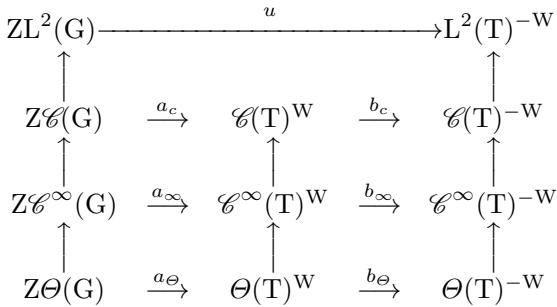
\includegraphics[keepaspectratio]{images/part003_8b0b3ceb.jpg}}

其中竖直箭头是典则包含映射，映射 \(b_{c}, b_{\infty}, b_{\Theta}\) 由 b 诱导，而 u 通过连续性延拓 \(b_{c} \circ a_{c}\)（§7, no. 4, Cor. 3 of Th. 2）。映射 u 和 \(b_{\Theta}\) 是双射（loc. cit.）；\(b_{\infty}\) 也是双射（Exerc. 5）；另一方面，\(b_{c}\) 一般不是满射（Exerc. 6）。

\section{紧李群在流形上的作用}

本节中，X 表示一个分离的、局部有限维的 \(C^{r}\) 类实流形（\(1 \leq r \leq \omega\)）。

\subsection{在紧集邻域中的流形嵌入}

引理 1. 设 T 和 T' 是两个拓扑空间，A 和 A' 分别是 T 和 T' 的紧子集，W 是 T × T' 中 A × A' 的一个邻域。存在 T 中 A 的开邻域 U 和 T' 中 A' 的开邻域 U'，使得 U × U' ⊂ W。

设 \(x \in \mathrm{A}\)；存在 \(\mathrm{U}_x\)（\(\mathrm{T}\) 的开子集）和 \(\mathrm{U}_x'\)（\(\mathrm{T}'\) 的开子集），使得 \(\{x\} \times \mathrm{A}' \subset \mathrm{U}_x \times \mathrm{U}_x' \subset \mathrm{W}\)：事实上，紧子集 \(\{x\} \times \mathrm{A}'\)（属于 \(\mathrm{T} \times \mathrm{T}'\)）可由有限个包含于 \(\mathrm{W}\) 中的开集覆盖，这些开集形如 \(\mathrm{U}_i \times \mathrm{U}_i'\)，且 \(x \in \mathrm{U}_i\)；只需取 \(\mathrm{U}_x = \bigcap_i \mathrm{U}_i\) 和 \(\mathrm{U}_x' = \bigcup_i \mathrm{U}_i'\) 即可。

由于 A 紧，存在 A 中的点 \(x_{1},\ldots,x_{m}\)，使得 \(A\subset\bigcup_{i}U_{x_{i}}\)；置 \(U=\bigcup_{i}U_{x_{i}}\) 和 \(U'=\bigcap_{i}U'_{x_{i}}\)。于是 \(A\times A'\subset U\times U'\subset W\)，引理得证。

本节余下部分中，Y 表示一个 \(C^{r}\) 类分离流形。

命题 1. 设 \(\varphi : \mathrm{X} \to \mathrm{Y}\) 是一个 \(\mathbf{C}^r\) 类态射，A 是 \(\mathrm{X}\) 的紧子集。下列条件等价：

\begin{enumerate}
\def\labelenumi{(\roman{enumi})}
\item
  \(\varphi\) 在 A 上的限制是单射，且 \(\varphi\) 在 A 的每一点处都是浸入；
\item
  存在 A 的一个开邻域 U，使得 \(\varphi\) 将 U 嵌入 Y 中。
\end{enumerate}

满足这些条件时，称 \(\varphi\) 在 A 的邻域中是嵌入。

证明 (i) 蕴含 (ii)，反向显然。假设 (i)，则存在包含 A 的 X 的一个开邻域 V，使得 \(\varphi\) 在 V 上是浸入（Differentiable and Analytic Manifolds, Results, 5.7.1）。记 \(\Gamma\) 为点 \((x,y)\)（属于 \(V \times V\)）且满足 \(\varphi(x) = \varphi(y)\) 的集合，记 \(\Delta\) 为 \(V \times V\) 中的对角线。则 \(\Delta\) 是 \(\Gamma\) 的开子集：事实上，对于所有 \(x \in V\)，存在 x 的一个开邻域 \(U_x\)，使得 \(\varphi\) 在 \(U_x\) 上是单射，即 \(\Gamma \cap (\mathrm{U}_x \times \mathrm{U}_x) = \Delta \cap (\mathrm{U}_x \times \mathrm{U}_x)\)。

由于 Y 是分离的，\(\varGamma\) 在 \(V \times V\) 中是闭的；因此 \(\varGamma - \varDelta\) 在 \(V \times V\) 中的补集 W 是开的。由假设，W 包含 \(A \times A\)；由引理 1，存在 V 中包含 A 的开子集 \(U'\)，使得 \(U' \times U' \subset W\)，也就是说，\(\varphi\) 在 \(U'\) 上的限制是单射。此外，存在 A 的一个开邻域 U，其闭包是紧的且包含于 \(U'\) 中（General Topology, Chap. I, §9, no. 7, Prop. 10）。于是 \(\varphi\) 诱导出从 \(\overline{U}\) 到 \(\varphi(\overline{U})\) 的同胚，因而也诱导出从 U 到 \(\varphi(U)\) 的同胚；由此 \(\varphi\) 在 U 上的限制是嵌入（Differentiable and Analytic Manifolds, Results, 5.8.3）。

命题 2. 假设流形 Y 是仿紧的；设 A 是 X 的子集，且 \(\varphi : X \to Y\) 是一个 \(C^r\) 类态射，它诱导出从 A 到 \(\varphi(A)\) 的同胚，并且在 A 的每一点处都是局部微分同胚。则存在 A 的一个开邻域 U，使得 \(\varphi\) 诱导出从 U 到 Y 的一个开子流形的同构。

必要时限制 X 和 Y 后，可假设 \(\varphi\) 是局部微分同胚且为满射。记 \(\sigma : \varphi(A) \to A\) 为 \(\varphi|A\) 的逆同胚。由于 Y 是可度量化的（Differentiable and Analytic Manifolds, Results, 5.1.6），\(\varphi(A)\) 有一个由仿紧邻域组成的基本邻域系；因此由 General Topology, Chap. XI，存在 Y 中 \(\varphi(A)\) 的一个开邻域 V 以及连续映射 \(s : V \to X\)，使得 s 与 \(\sigma\) 在 \(\varphi(A)\) 上一致，并且 \(\varphi(s(y)) = y\) 对所有 \(y \in V\) 成立。此外，s 在拓扑意义下是局部微分同胚的，故 \(s(V)\) 是包含 A 的开集 U。于是 \(\varphi\) 诱导出从 U 到 V 的同胚 \(\varphi'\)；由 Differentiable and Analytic Manifolds, Results, 5.7.8，\(\varphi'\) 是同构。

本节余下部分中，假设 \(r \neq \omega\)。

命题 3. 设 A 是 X 的紧子集。在 A 的邻域中为嵌入的态射 \(\varphi \in \mathcal{C}^{r}(X;Y)\) 所成的集合 P，在 \(\mathcal{C}^{r}(X;Y)\) 中关于紧 \(C^{r}\) 收敛的拓扑（\(\S\) 6, no. 4）下是开的。

显然，只需对 \(r = 1\) 证明该命题。

\begin{enumerate}
\def\labelenumi{\alph{enumi})}
\tightlist
\item
  先证明 \(\mathcal{C}^{1}(\mathrm{X};\mathrm{Y})\) 的子集 J 是开的，其中 J 由在 A 的每一点处为浸入的态射组成。考虑映射 \(j_{\mathrm{A}}:\mathcal{C}^{1}(\mathrm{X};\mathrm{Y})\times\mathrm{A}\to\mathrm{J}^{1}(\mathrm{X};\mathrm{Y})\)，满足 \(j_{\mathrm{A}}(\varphi,x)=j_{x}^{1}(\varphi)\)（Differentiable and Analytic Manifolds, Results, 12.1）。
\end{enumerate}

由 \(\mathcal{C}^1 (\mathrm{X};\mathrm{Y})\) 上拓扑的定义，映射 \(\tilde{j}_{\mathrm{A}}:\varphi \to j_{\mathrm{A}}(\varphi ,.)\) 从 \(\mathcal{C}^1 (\mathrm{X};\mathrm{Y})\) 到 \(\mathcal{C}(\mathrm{A};\mathrm{J}^1 (\mathrm{X};\mathrm{Y}))\) 是连续的；由此根据 General Topology, Chap. X, §3, no. 4, Th. 3，\(j_{\mathrm{A}}\) 是连续的。

另一方面，设 M 是 \(\mathrm{J}^{1}(\mathrm{X};\mathrm{Y})\) 中的喷流 j 的集合，这些喷流的切映射 \(\mathrm{T}(j):\mathrm{T}_{\mathbf{s}(j)}(\mathrm{X})\to\mathrm{T}_{\mathbf{b}(j)}(\mathrm{Y})\)（Differentiable and Analytic Manifolds, Results, 12.3.4）是单射。集合 M 在 \(\mathrm{J}^{1}(\mathrm{X};\mathrm{Y})\) 中是开的；事实上，只需在 X 是有限维向量空间 E 的开子集且 Y 是 Banach 空间 F 的开子集时验证该断言；根据 Differentiable and Analytic Manifolds, Results, 12.3.1，这归结为证明单射连续线性映射的集合在 \(\mathcal{L}(\mathrm{E};\mathrm{F})\) 中是开的，而这由 Spectral Theory, Chap. III, §2, no. 7, Prop. 16 得到。

由前述结果，集合 \(j_{\mathrm{A}}^{-1}(\mathrm{M})\) 在 \(\mathcal{C}^{1}(\mathrm{X};\mathrm{Y})\times\mathrm{A}\) 中是开的，故其补集 F 是闭的。由于 A 紧，投影 \(\mathrm{pr}_{1}:\mathcal{C}^{1}(\mathrm{X};\mathrm{Y})\times\mathrm{A}\to\mathcal{C}^{1}(\mathrm{X};\mathrm{Y})\) 是真的态射，因而是闭映射；所以集合 J（等于 \(\mathcal{C}^{1}(\mathrm{X};\mathrm{Y})-\mathrm{pr}_{1}(\mathcal{F})\)）在 \(\mathcal{C}^{1}(\mathrm{X};\mathrm{Y})\) 中是开的。

\begin{enumerate}
\def\labelenumi{\alph{enumi})}
\setcounter{enumi}{1}
\tightlist
\item
  设 H 是 \(J \times A \times A\) 的子集，由元素 \((f, x, y)\) 组成，满足 \(f(x) = f(y)\)。显然 H 包含 \(J \times \Delta\)，其中 \(\Delta\) 表示乘积 \(A \times A\) 中的对角线；我们证明 \(H' = H - (J \times \Delta)\) 在 \(J \times A \times A\) 中是闭的。由于 P 是 J 中 \(H'\) 在真的投影 \(pr_{1}: J \times A \times A \to J\) 下的像的补集，这将推出该命题。
\end{enumerate}

由于 \(\mathcal{C}^{1}(\mathrm{X};\mathrm{Y})\) 的拓扑比紧收敛拓扑精细，映射 \((\varphi,x)\mapsto\varphi(x)\) 从 \(\mathcal{C}^{1}(\mathrm{X};\mathrm{Y})\times\mathrm{A}\) 到 Y 是连续的（General Topology, Chap. X, §3, no. 4, Cor. 1 of Th. 3）；由此 H 在 \(J\times A\times A\) 中是闭的。因此只需证明 \(J\times\Delta\) 在 H 中是开的，换言之，对于所有 \(\varphi\in J\) 和所有 \(x\in A\)，存在一个邻域 \(\Omega\)（J 中 \(\varphi\) 的邻域）以及 X 中 x 的一个邻域 B，使得对于任意态射 \(\psi\)（属于 \(\Omega\)），\(\psi\) 在 \(A\cap B\) 上的限制是单射。

因此，该命题由下列引理推出：

引理 2. 设 x 是 X 的一点，\(\varphi: X \to Y\) 是一个 \(C^{1}\) 类态射，且在 x 处是浸入。存在一个邻域 \(\Omega\)（\(\varphi\) 在 \(\mathcal{C}^{1}(X;Y)\) 中的邻域）以及 X 中 x 的一个邻域 B，使得对于所有 \(\psi \in \Omega\)，\(\psi\) 在 B 上的限制是单射。

设 U 是 x 的一个相对紧开邻域，它同构于某个有限维向量空间，并且 \(\varphi(\overline{\mathrm{U}})\) 包含于图册的定义域 V 中。由集合 \(\Omega_{0}\)（它由满足 \(\psi\in\mathcal{C}^{1}(\mathrm{X};\mathrm{Y})\) 且 \(\psi(\overline{\mathrm{U}})\subset\mathrm{V}\) 的态射组成）在 \(\mathcal{C}^{1}(\mathrm{X};\mathrm{Y})\) 中是开的，且限制映射 \(\Omega_{0}\to\mathcal{C}^{1}(\mathrm{U};\mathrm{V})\) 是连续的；因此只需在 X=U 且 Y=V 时证明该引理，换言之，可假设 X 是有限维向量空间而 Y 是 Banach 空间。在 X 和 Y 上选取范数。

线性映射 \(\mathrm{D}\varphi(x):\mathrm{X}\to\mathrm{Y}\) 是单射；记其余范数为 q（Spectral Theory, Chap. III, §2, no. 6），于是按定义，有 \(\|\mathrm{D}\varphi(x).t\|\geq q\|t\|\) 对所有 \(t\in X\) 成立。取 \(\varepsilon\in R\) 使得 \(0<\varepsilon<q/2\)，并取一个以 x 为中心的闭球 B，使得 \(\|\mathrm{D}\varphi(u)-\mathrm{D}\varphi(x)\|\leq\varepsilon\) 对所有 \(u\in B\) 成立。记 \(\Omega\) 为 \(\mathcal{C}^{1}(\mathrm{X};\mathrm{Y})\) 中的态射 \(\psi\) 所成的子集，其中满足 \(\|\mathrm{D}\psi(u)-\mathrm{D}\varphi(u)\|\leq\varepsilon\) 对所有 \(u\in B\) 成立；按 \(\mathcal{C}^{1}(\mathrm{X};\mathrm{Y})\) 拓扑的定义，它是开的。对于 \(\psi\in\Omega\)，置 \(\psi_{0}=\psi-\mathrm{D}\varphi(x)\)。有 \(\|\mathrm{D}\psi_{0}(u)\|\leq2\varepsilon\) 对所有 \(u\in B\) 成立，因而有 \(\|\psi_{0}(u)-\psi_{0}(v)\|\leq2\varepsilon\|u-v\|\) 对 B 中所有 u 和 v 成立（Differentiable and Analytic Manifolds, Results, 2.2.3）。由此

\[
\| \psi (u) - \psi (v) \| \geq \| \mathrm{D} \varphi (x). (u - v) \| - \| \psi_ {0} (u) - \psi_ {0} (v) \| \geq (q - 2 \varepsilon) \| u - v \|.
\]

所以 \(\psi\) 在 B 上的限制是单射，引理得证。

命题 4. 设 A 是 X 的紧子集。存在有限维向量空间 E 以及一个态射 \(\varphi \in \mathcal{C}^r (\mathrm{X};\mathrm{E})\)（\(r\neq \omega\)），使得它在 A 的邻域中是嵌入。

设 \((\mathrm{U}_{i},\varphi_{i},\mathrm{E}_{i})_{i\in\mathrm{I}}\) 是 X 的一个有限图册族，其定义域覆盖 A。我们将 \(\varphi_{i}\) 延拓为从 X 到 \(E_{i}\) 的映射（仍记作 \(\varphi_{i}\)），规定 \(\varphi_{i}(x)=0\)（\(x\notin U_{i}\)）。设 \((\mathrm{V}_{i})_{i\in\mathrm{I}}\) 是由 X 的开子集组成的 A 的一个覆盖，使得 \(\overline{\mathrm{V}}_{i}\subset\mathrm{U}_{i}\) 对所有 \(i\in\mathrm{I}\) 成立（这种覆盖的存在性由 General Topology, Chap. IX, §4, no. 3, Cor. 1 of Th. 3 得到：将该结果应用于紧空间 \(X'\) 及 \(X'\) 的覆盖，后者由开集 \(U_{i}\)（\(i\in\mathrm{I}\)）和 \(X'-\mathrm{A}\) 组成；X' 是通过向 X 添加无穷远点得到的空间）。对于所有 \(i\in\mathrm{I}\)，取 \(\alpha_{i}\) 为 X 上的一个 \(C^{r}\) 类数值函数，它在 \(V_{i}\) 的每一点处等于 1，且其支集包含于 \(U_{i}\)（Differentiable and Analytic Manifolds, Results, 5.3.6）。

考虑由下式定义的映射 \(\varphi : \mathrm{X} \to \bigoplus_{i \in \mathrm{I}} (\mathrm{E}_i \oplus \mathbf{R})\)

\[
\varphi (x) = (\alpha_ {i} (x) \varphi_ {i} (x), \alpha_ {i} (x)) _ {i \in I}.
\]

对于所有 \(i \in I\)，映射 \(\alpha_{i}\varphi_{i}\) 是 \(C^{r}\) 类的（因为它在 \(U_{i}\) 以及 \(\alpha_{i}\) 的支集的补集上的限制都是如此），且其在 \(V_{i}\) 上的限制是嵌入；由此 \(\varphi\) 是 \(C^{r}\) 类态射，并且在 A 的每一点处都是浸入。我们证明 \(\varphi\) 在 A 上的限制是单射。设 x、y 是 A 中满足 \(\varphi(x) = \varphi(y)\) 的两点，并取 \(i \in I\)，使得 \(x \in V_{i}\)。则 \(\alpha_{i}(x) = 1\)，所以 \(\alpha_{i}(y) = 1\)，这推出 \(y \in U_{i}\)；但还有 \(\varphi_{i}(x) = \varphi_{i}(y)\)，故 x = y，因为 \(\varphi_{i}\) 将 \(U_{i}\) 嵌入 \(E_{i}\)。

可以证明 \(^{9}\)，每个分离的、无穷远可数且纯维数为 n 的流形都能嵌入 \(R^{2n}\)；较弱的结果见 cf.~Exercise 2。

\subsection{等变嵌入定理}

本节中假设 \(r \neq \omega\)。

引理 3. 设 G 是一个在拓扑空间 X 上连续作用的紧拓扑群；设 A 是 X 的子集，在 G 的作用下稳定，W 是 A 的一个邻域。则存在 A 的一个开邻域 V，在 G 的作用下稳定且包含于 W 中。

置 \(\mathrm{F} = \mathrm{X} - \mathrm{W}\) 和 \(\mathrm{V} = \mathrm{X} - \mathrm{GF}\)。则 \(\mathrm{V}\) 是开的（General Topology, Chap. III, §4, no. 1, Cor. 1 of Prop. 1），在 \(\mathrm{G}\) 的作用下稳定，且 \(\mathrm{A} \subset \mathrm{V} \subset \mathrm{W}\)。

定理 1. 设 G 是紧李群，\((g,x)\mapsto gx\) 是 G 在 X 上的 \(C^{r}\) 类左作用律，A 是 X 的紧子集。存在 G 在有限维向量空间 E 上的解析线性表示 \(\rho\)、一个态射 \(\varphi:X\to E\)（为 \(C^{r}\) 类，与 G 的作用相容）以及 A 的一个开邻域 U，在 G 的作用下稳定，使得 \(\varphi\) 在 U 上的限制是嵌入。

用紧集 GA 替换 A 后，可归结为 A 在 G 的作用下稳定的情形。

设 \(E_0\) 是一个有限维向量空间，使得 \(\mathcal{C}^r(\mathrm{X};\mathrm{E}_0)\) 中存在在 A 的邻域中为嵌入的元素（no. 1, Prop. 4）；具有此性质的态射所成的集合 \(\mathcal{P}\) 是 \(\mathcal{C}^r(\mathrm{X};\mathrm{E}_0)\) 的非空开子集（no. 1, Prop. 3）。考虑紧群 G 在空间 \(\mathcal{C}^r(\mathrm{X};\mathrm{E}_0)\) 上的连续线性表示（§6, no. 4, Lemma 4）。由 Peter–Weyl 定理（Spectral Theory, in preparation），在 G 的作用下稳定的有限维子空间之并在 \(\mathcal{C}^r(\mathrm{X};\mathrm{E}_0)\) 中稠密；因此，存在元素 \(\varphi_0\) 属于 \(\mathcal{P}\)，使得映射 \(x \mapsto \varphi_0(gx)\)（\(g \in G\)）生成有限维向量子空间 \(E_1\)，它是 \(\mathcal{C}^r(\mathrm{X};\mathrm{E}_0)\) 的子空间，该子空间显然在 G 的作用下稳定。

取 E 为空间 \(\operatorname{Hom}_{\mathbf{R}}(\mathrm{E}_{1},\mathrm{E}_{0})\)，取 \(\rho\) 为 G 在 E 上由其在 \(E_{1}\) 上的作用诱导的表示，并令 \(\varphi:X\to E\) 为将 \(x\in X\) 赋予线性映射 \(\psi\mapsto\psi(x)\)（从 \(E_{1}\) 到 \(E_{0}\)）的映射。这是 \(C^{r}\) 类态射；对于 \(x\in X\)、\(g\in G\)、\(\psi\in E_{1}\)，有（记 \(\tau(g)\) 为 X 的自同构 \(x\mapsto gx\)）：

\[
\varphi (g x) (\psi) - \psi (g x) = \varphi (x) (\psi \circ \tau (g)) = (\rho (g) \varphi (x)) (\psi).
\]

令 \(\alpha : \mathrm{Hom}_{\mathbf{R}}(\mathrm{E}_1, \mathrm{E}_0) \to \mathrm{E}_0\) 为线性映射 \(u \mapsto u(\varphi_0)\)；有 \(\alpha \circ \varphi = \varphi_0\)，所以 \(\varphi\) 在 A 的邻域中是嵌入（因为 \(\varphi_0\) 是嵌入）。因此存在 A 的一个开邻域 U，使得 \(\varphi\) 在 U 上的限制是嵌入；由引理 3 可将 U 选为在 G 的作用下稳定的，定理得证。

推论 1. 假设 X 是紧的。存在 G 在有限维向量空间 E 上的解析线性表示 \(\rho\) 以及一个嵌入 \(\varphi: X \to E\)，使得 \(\varphi(gx) = \rho(g)\varphi(x)\) 对 \(g \in G, x \in X\) 成立。

推论 2. 设 H 是 G 的闭子群。存在 G 在有限维向量空间 E 上的解析线性表示以及一点 \(v \in E\)，其固定子群为 H。

将推论 1 应用于 G 在紧流形 G/H 上的典则作用。这给出解析线性表示 \(\rho: \mathrm{G} \to \mathbf{GL}(\mathrm{E})\) 以及嵌入 \(\varphi: \mathrm{G} / \mathrm{H} \to \mathrm{E}\)，使得 \(\varphi(gx) = \rho(g)\varphi(x)\)，其中 \(g \in \mathrm{G}, x \in \mathrm{G} / \mathrm{H}\)。令 \(\bar{e} \in \mathrm{G} / \mathrm{H}\) 为 \(e \in \mathrm{G}\) 的等价类，并令 \(v = \varphi(\bar{e})\) 为其像。对于所有 \(g \in \mathrm{G}\)，有 \(\rho(g)v = v \Longleftrightarrow \varphi(g\bar{e}) = \varphi(\bar{e}) \Longleftrightarrow g\bar{e} = \bar{e} \Longleftrightarrow g \in \mathrm{H}\)。

推论 3. 假设 X 是仿紧的。存在实希尔伯特空间 E、G 在 E 上的连续酉表示 \({}^{10}\) \(\rho\) 以及一个嵌入 \(\varphi: X \to E\)（为 \(C^{r}\) 类），使得 \(\varphi(gx) = \rho(g)\varphi(x)\) 对所有 \(g \in G\) 和所有 \(x \in X\) 成立。

空间 X/G 是局部紧的（General Topology, Chap. III, §4, no. 5, Prop. 11）。它的连通分支是 X 的连通分支的像，而 X 的连通分支在无穷远处可数（General Topology, Chap. I, §9, no. 10, Th. 5）；因此这些像自身也在无穷远处可数，从而 X/G 是仿紧的（loc. cit.）。所以存在 X/G 的一个局部有限覆盖 \((\mathrm{U}_{\alpha}^{\prime})_{\alpha\in\mathrm{I}}\)，其成员为相对紧开集；还存在覆盖 \((\mathrm{V}_{\alpha}^{\prime})_{\alpha\in\mathrm{I}}\)，使得 \(\overline{V}_{\alpha}^{\prime}\subset U_{\alpha}^{\prime}\) 对所有 \(\alpha\in I\) 成立（General Topology, Chap. IX, §4, no. 3, Cor. 1 of Th. 3）。取逆像后，得到 X 的两个局部有限覆盖 \((\mathrm{U}_{\alpha})_{\alpha\in\mathrm{I}}\) 和 \((\mathrm{V}_{\alpha})_{\alpha\in\mathrm{I}}\)，其成员为在 G 下稳定的相对紧开集，并且 \(\overline{V}_{\alpha}\subset U_{\alpha}\) 对所有 \(\alpha\in I\) 成立。

对于所有 \(\alpha \in \mathrm{I}\)，存在一个表示 \(\rho_{\alpha}\)，它作用在有限维实向量空间 \(\mathrm{E}_{\alpha}\) 上，以及一个与 G 的作用相容的态射 \(\varphi_{\alpha} \in \mathcal{C}^r (\mathrm{X};\mathrm{E}_{\alpha})\)，且其在 \(\mathrm{U}_{\alpha}\) 上的限制是嵌入（定理 1）。对于 \(\alpha \in \mathrm{I}\)，取一个 \(a_{\alpha}\)，它是 X 上的 \(\mathrm{C}^r\) 类数值函数，在 \(\mathrm{V}_{\alpha}\) 上等于 1，在 \(\mathrm{U}_{\alpha}\) 外等于 0（Differentiable and Analytic Manifolds, Results, 5.3.6）。置 \(b_{\alpha}(x) = \int_{\mathrm{G}} a_{\alpha}(gx) dg\) 对于 \(x \in \mathrm{X}\) 成立。函数 \(b_{\alpha}\) 是 \(\mathrm{C}^r\) 类的，在 G 下不变（§6, no. 4, Cor. 2），在 \(\mathrm{V}_{\alpha}\) 上等于 1，在 \(\mathrm{U}_{\alpha}\) 外等于 0。在每个 \(\mathrm{E}_{\alpha}\) 上取一个 G-不变的希尔伯特内积（§1, no. 1），并在 R 上取其典则希尔伯特结构；令 E 为族 \((\mathrm{E}_{\alpha} \oplus \mathbf{R})_{\alpha \in \mathrm{I}}\) 的希尔伯特和，并令 \(\rho\) 为 G 在 E 上由各 \(\rho_{\alpha}\) 以及 G 在 R 上的平凡作用诱导的表示。对于 \(x \in \mathrm{X}\)，置 \(\varphi(x) = (b_{\alpha}(x)\varphi_{\alpha}(x), b_{\alpha}(x))_{\alpha \in \mathrm{I}}\)。则 \(\varphi\) 是从 X 到 E 的 \(\mathrm{C}^r\) 类态射，与 G 的作用相容；如命题 4 的证明（no. 1）中那样验证 \(\varphi\) 是嵌入，即得该推论。

\subsection{管与横截面}

引理 4. 设 H 是紧李群，\(\rho : \mathrm{H} \to \mathbf{GL}(\mathrm{V})\) 是 H 在有限维实向量空间 V 上的连续（因而解析）表示，W 是 V 中原点的一个邻域。存在原点的一个开邻域 B，它包含于 W 且在 H 的作用下稳定；还存在一个解析同构 \(u: \mathrm{V} \to \mathrm{B}\)，与 H 的作用相容，并满足 \(u(0) = 0\) 和 \(\mathrm{Du}(0) = \mathrm{Id}_{\mathrm{V}}\)。

在 V 上选取一个 H-不变内积（§1, no. 1）。存在实数 \(r > 0\)，使得半径为 \(r\) 的开球 B 包含于 W 中；它显然在 H 的作用下稳定。置 \(u(v) = r(r^2 + \|v\|^2)^{-1/2} v\)，对所有 \(v \in V\) 成立；于是 \(u\) 是从 V 到 B 的双射解析映射，与 H 的作用相容，且其逆映射 \(w \mapsto r(r^2 - \|w\|^2)^{-1/2} w\) 是解析的。此外，\(u(0) = 0\) 且 \(\mathrm{D}u(0) = \mathrm{Id}_{\mathrm{V}}\)。

命题 5. 设 H 是紧李群，\((h,x)\mapsto hx\) 是 H 在 X 上的 \(C^{r}\) 类左作用律，x 是 X 中在 H 的作用下固定的一点。则群 H 在线性地作用于向量空间 \(T=T_{x}(X)\) 上；存在一个开嵌入 \(\varphi:T\to X\)，为 \(C^{r}\) 类，与 H 的作用相容，并满足 \(\varphi(0)=x\) 且 \(T_{0}(\varphi)\) 是 T 的恒等映射。

设 \((\mathrm{U},\psi,\mathrm{E})\) 是 X 在 x 处的一个图册，使得 U 在 H 的作用下稳定（no. 2, Lemma 3）且 \(\psi(x)=0\)。通过 \(\mathrm{T}_{x}(\psi)\) 将 E 与 T 识别，并置

\[
\psi^ {\sharp} (y) = \int_ {\mathrm{H}} h. \psi (h ^ {- 1} y) d h \quad \text { for } y \in \mathrm{U},
\]

其中 dh 是 H 上总质量为 1 的 Haar 测度。

于是（§6, no. 4, Cor. 1）\(\psi^{\sharp}\) 是从 U 到 T 的 \(\mathrm{C}^r\) 类态射，与 H 的作用相容，并满足 \(\psi^{\sharp}(x) = 0\) 和 \(d_x\psi^\sharp = \mathrm{Id}_\mathrm{T}\)。因此存在一个开集 \(\mathrm{U}' \subset \mathrm{U}\)，包含 \(x\)，以及 T 中 0 的一个开邻域 V，使得 \(\psi^{\sharp}\) 诱导出同构 \(\theta: \mathrm{U}' \to \mathrm{V}\)。必要时限制 \(\mathrm{U}'\) 和 V，可假设它们在 H 的作用下稳定，并且存在与 H 的作用相容的同构 \(u: \mathrm{T} \to \mathrm{V}\)（引理 4）。现在只需取 \(\varphi = \theta^{-1} \circ u\)。

回忆（Differentiable and Analytic Manifolds, Results, 6.5.1），若 G 是李群，H 是 G 的李子群，且 Y 是 H 在其上左作用的流形，则记 \(G \times^{H}Y\) 为乘积流形 \(G \times Y\) 关于 H 的右作用 \(((g,y),h) \mapsto (gh,h^{-1}y)\) 的商；这是一个李群 G 在其上自然地左作用的流形；投影 \(G \times^{H}Y \to G/H\) 是纤维为 Y 的丛。此外，若 Y 是 H 在线性作用的有限维向量空间，则 \(G \times^{H}Y\) 自然具有以 G/H 为底空间的向量 G-丛结构（Differentiable and Analytic Manifolds, Results, 7.10.2）。

设 G 是一个在流形 X 上真作用的李群（General Topology, Chap. III, §4, no. 1, Def. 1），且作用律 \((g, x) \mapsto gx\) 是 \(C^{r}\) 类的。则对于 X 中的每一点 x，x 的轨道 Gx 是 X 的闭子流形，同构于李齐性空间 \(G/G_{x}\)，其中 \(G_{x}\) 是 G 中 x 的固定子群（cf.~Chap. III, §1, no. 7, Prop. 14 (ii), and General Topology, Chap. III, §4, no. 2, Prop. 4）；后者是紧李群（loc. cit.）。

命题 6. 假设流形 X 是仿紧的；设 x 是 X 中的一点，\(G_{x}\) 是其固定子群。存在有限维解析线性表示 \(\tau: G_{x} \to \mathbf{GL}(W)\)，以及一个开嵌入 \(\alpha: G \times ^{G_{x}} W \to X\)，为 \(C^{r}\) 类，与 G 的作用相容，并将 \((e,0) \in G \times W\) 的等价类映到 x。

置 \(T = T_{x}(X)\)。设 W 是 T 中 \(T_{x}(Gx)\) 的一个补子空间，在 \(G_{x}\) 的作用下稳定（例如，取 \(T_{x}(Gx)\) 相对于 T 上 \(G_{x}\)-不变内积的正交补）。另一方面，设 \(\varphi : T \to X\) 是具有命题 5 所述性质的态射（相对于 \(H = G_{x}\)）。考虑态射 \(\lambda : G \times W \to X\)，其定义为 \(\lambda(g, w) = g\varphi(w)\)。它通过取商诱导出态射 \(\mu : G \times^{G_{x}}W \to X\)，为 \(C^{r}\) 类，与 G 的作用相容，并将 \((e, 0)\) 的等价类 z 映到 x。

我们证明 \(\mu\) 在点 \(z\) 处是局部微分同胚的。有

\[
\begin{array}{c} \dim (\mathrm{G} \times {} ^ {\mathrm{G} _ {x}} \mathrm{W}) = \dim (\mathrm{G}) + \dim (\mathrm{W}) - \dim (\mathrm{G} _ {x}) \\ = \dim (\mathrm{G} x) + \dim (\mathrm{W}) = \dim (\mathrm{T}), \end{array}
\]

所以只需证明 \(\mu\) 在 \(z\) 处是下沉映射，或等价地，\(\lambda\) 在 \((e,0)\) 处是下沉映射。但是，切映射 \(\mathrm{T}_{(e,0)}(\lambda):\mathrm{T}_e(\mathrm{G})\oplus \mathrm{W}\to \mathrm{T}\) 等于 \(\mathrm{T}_e(\rho (x)) + i\)，其中 \(\rho (x)\) 是轨道映射 \(g\mapsto gx\)，而 \(i\) 是从 W 到 T 的典则嵌入；由于 \(\operatorname {Im}\operatorname {T}_e(\rho (x)) = \operatorname {T}_x(\operatorname {G}x)\)，切映射 \(\mathrm{T}_{(e,0)}(\lambda)\) 是满射，且 \(\mu\) 在 \(z\) 处是局部微分同胚的。

我们将证明，存在一个开邻域 \(\Omega\)，它是 \(Gz\) 在 \(G \times ^{G_x}W\) 中的邻域，在 \(G\) 的作用下稳定，使得 \(\mu\) 将 \(\Omega\) 同构到 \(X\) 的一个开子集上。这将推出该命题：事实上，\(\Omega\) 在 \(G \times W\) 中的逆像在 \(G\) 的作用下稳定，因而形如 \(G \times B\)，其中 \(B\) 是 \(W\) 中包含原点且在 \(G_x\) 的作用下稳定的开子集；必要时限制 \(\Omega\)，可假设存在同构 \(u: W \to B\)，与 \(G_x\) 的作用相容（引理 4）。显然，复合态射 \(\alpha: G \times ^{G_x}W \xrightarrow{(\text{Id}, u)} G \times ^{G_x}B \xrightarrow{\mu} X\) 满足命题中的条件。

因此，该命题是下列引理的推论：

引理 5. 设 Z 是一个 \(C^{r}\) 类分离流形，带有一个左作用律 \(m: G \times Z \to Z\)，为 \(C^{r}\) 类，且 \(\mu: Z \to X\) 是一个与 G 的作用相容的（\(C^{r}\) 类）态射。设 z 是 Z 中的一点，且 \(x = \mu(z)\)。假设 \(\mu\) 在 z 处是局部微分同胚的，且 G 中 z 的固定子群等于 x 的固定子群 \(G_{x}\)。则存在一个开邻域 \(\Omega\)，它是轨道 Gz 的邻域，在 G 的作用下稳定，使得 \(\mu\) 将 \(\Omega\) 同构到 X 的一个开子集上。

由于 \(\mu\) 与 G 的作用相容，它在 Gz 的每一点处都是局部微分同胚的；由于典则映射 \(G/G_{x} \rightarrow Gx\) 是同胚，由 \(\mu\) 诱导的从 Gz 到 Gx 的映射也是同胚。因此由 no. 1 的命题 2 可知，Z 中存在 Gz 的一个开邻域 U，使得 \(\mu\) 将 U 开嵌入 X。

由于 G 在 X 上真作用，存在 x 的一个开邻域 V 以及 G 的一个紧子集 K，使得当 \(gV \cap V = \varnothing\)（\(g \notin K\) 时）；特别地，\(e \in K\)。集合 \(W_{1}\) 由 Z 中满足 \(y \in Z\) 且 \(Ky \subset U\) 的点组成，是开的：事实上，\(Z - W_{1}\) 是闭集 \((\mathrm{K} \times \mathrm{Z}) - m^{-1}(\mathrm{U})\) 在真投影 \(pr_{2}: K \times Z \to Z\) 下的像。置 \(W = W_{1} \cap \mu^{-1}(V)\)；这是 Z 的一个包含 z 的开子集，并满足下列条件：

\begin{enumerate}
\def\labelenumi{(\roman{enumi})}
\item
  KW \(\subset\) U，特别是 W \(\subset\) U；
\item
  \(\mu(\mathrm{W}) \subset \mathrm{V}.\)
\end{enumerate}

置 \(\Omega = \mathrm{GW}\)，并考虑 \(\mu\) 在 \(\Omega\) 上的限制。这是一个局部微分同胚态射，因为 \(\Omega\) 的每一点都在 \(\mathbf{G}\) 的作用下与 \(\mathbf{U}\) 中的一点共轭。我们证明它是单射：设 \(g, h\) 属于 \(\mathbf{G}\)，\(u, v\) 属于 \(\mathbf{W}\)，且满足 \(\mu(gu) = \mu(hv)\)。置 \(k = g^{-1}h\)；则 \(\mu(u) = k\mu(v)\)，由 (ii) 得 \(k \in \mathbf{K}\)。但由 (i)，\(kv\) 和 \(u\) 都属于 \(\mathbf{U}\)；于是 \(u = kv\)，因为 \(\mu\) 在 \(\mathbf{V}\) 上的限制是单射，所以 \(gu = hv\)。因此 \(\mu\) 在 \(\Omega\) 上的限制是单射，从而根据 Differentiable and Analytic Manifolds, Results, 5.7.8，它是到 \(\mathbf{X}\) 的一个开子流形上的同构，证明完成。

在命题 6 的条件下，\(\alpha\) 的像是轨道 A 的点 \(x\) 的一个开邻域 T，它带有以 A 为底空间的向量丛结构，且零截面就是轨道 A 本身。对于每个点 \(a \in \mathrm{A}\)，该向量丛的纤维 \(\mathrm{Y}_a\) 是 X 的子流形，在固定子群 \(\mathrm{G}_a\)（对应点 \(a\)）的作用下稳定，并且有一个从 \(\mathrm{G} \times^{\mathrm{G}_a}\mathrm{Y}_a\) 到 X 的态射，它将 \((g,y) \in \mathrm{G} \times \mathrm{Y}_a\) 的等价类映到 \(gy \in \mathrm{X}\)，并且它诱导出一个 \(\mathrm{C}^r\) 类态射，从 \(\mathrm{G} \times^{\mathrm{G}_a}\mathrm{Y}_a\) 到 T。称 \(\mathrm{Y}_a\) 为管 T 在 \(a\) 处的横截面。注意，在 \(a\) 处，\(\mathrm{Y}_a\) 的切空间典则同构于 \(\mathrm{Y}_a\)，并且它是 \(\mathrm{T}_a(\mathrm{A})\) 在 \(\mathrm{T}_a(\mathrm{X})\) 中的一个补空间；因此，以 A 为底空间的向量丛 T 典则同构于 A 在 X 中的法丛（Differentiable and Analytic Manifolds, Results, 8.1.3）。

\subsection{轨道类型}

设 \(G\) 是在分离拓扑空间 \(E\) 上连续作用的拓扑群。对于每一点 \(x\)（属于 \(E\)），记 \(G_x\) 为 \(x\) 在 \(G\) 中的固定子群，并假设典则映射 \(G / G_x \to Gx\) 是同胚；以下两种情形尤其满足此条件：

\begin{enumerate}
\def\labelenumi{\alph{enumi})}
\item
  G 和 E 的拓扑都是离散的；
\item
  G 在 E 上真作用（General Topology, Chap. III, §4, no. 2, Prop. 4），例如 G 是紧的（General Topology, Chap. III, §4, no. 1, Prop. 2）。
\end{enumerate}

记 \(\mathcal{T}\) 为 G 的闭子群的共轭类集合。对于每个 \(x\in \mathrm{E}\)，称 \(x\) 的轨道类型（有时简称 \(x\) 的类型）为 \(\mathrm{G}_x\) 在 \(\mathcal{T}\) 中的类；同一轨道上的两点具有相同的轨道类型（Algebra, Chap. I, §5, no. 2, Prop. 2）；两个轨道具有相同类型，当且仅当它们作为 G-集合同构（Algebra, Chap. I, §5, no. 5, Th. 1）。对于每个 \(t\in \mathcal{T}\)，记 \(\mathrm{E}_{(t)}\) 为 E 中类型为 \(t\) 的点的集合，即类型为 \(t\) 的轨道之并；这是 E 的稳定子集。对于 \(\mathrm{H}\in t\)，也将 \(\mathrm{E}_{(\mathrm{H})}\) 记作 \(\mathrm{E}_{(t)}\)；例如，\(\mathrm{E}_{(\mathrm{G})}\) 是由 G 固定的点组成的 E 的闭子空间。

在 T 上定义如下预序关系：

\(t \leq t'\Longleftrightarrow\) 存在 \(\mathrm{H} \in t\) 和 \(\mathrm{H}' \in t'\)，使得 \(\mathrm{H} \supset \mathrm{H}'\)。

设 \(\Omega\) 和 \(\Omega'\) 是 G 在 E 上的两个轨道，\(t\) 和 \(t'\) 分别是它们的类型；则 \(t \leq t'\) 当且仅当存在从 \(\Omega'\) 到 \(\Omega\) 的 G-态射（必为满射且连续）。

设 \(x, x'\) 属于 E，\(t, t'\) 是它们的类型；则 \(t \leq t'\) 当且仅当存在 \(a \in G\)，使得 \(aG_{x'}a^{-1} \subset G_x\)。

引理 6. 设 G 是李群。

\begin{enumerate}
\def\labelenumi{\alph{enumi})}
\item
  \(\mathbf{G}\) 的每个递降紧子群序列都是最终稳定的。
\item
  设 H 和 \(H'\) 是 G 的两个紧子群，满足 \(H \subset H'\)，且存在从 \(H'\) 到 H 的（拓扑群）同构。则 \(H = H'\)。
\item
  对于关系 \(t \leq t'\)，集合 \(\mathcal{T}\) 是一个诺特有序集（Theory of Sets, Chap. III, §6, no. 5, text preceding Prop. 7）。
\item
  设 \((\mathrm{H}_{i})_{i\geq1}\) 是 G 的一个递降紧子群序列；这些子群都是 G 的李子群（Chap. III, §8, no. 2, Th. 2）。整数序列 \((\dim\mathrm{H}_{i})_{i\geq1}\) 递降，因而最终稳定，所以存在整数 N，使得子群 \(H_{i}\) 在 \(i\geq N\) 时具有相同的单位元连通分支。于是正整数序列 \((\mathrm{H}_{i}:(\mathrm{H}_{i})_{0})_{i\geq N}\) 递降且最终稳定，因此当 i 充分大时 \(H_{i}=H_{i+1}\)。
\item
  设 \(f\) 是从 \(\mathrm{H}'\) 到 \(\mathrm{H}\) 的同构。序列 \((f^n(\mathrm{H}))_{n\geq 0}\) 是 \(\mathrm{G}\) 的递降紧子群序列，故 \(f^n(\mathrm{H}) = f^{n + 1}(\mathrm{H})\) 对充分大的 \(n\) 成立，由 \(a\) 可知。由于 \(f\) 是同构，这推出 \(f(\mathrm{H}) = \mathrm{H} = f(\mathrm{H}')\)，所以 \(\mathrm{H} = \mathrm{H}'\)。
\item
  设 \(t, t' \in \mathcal{T}\) 满足 \(t \leq t'\) 且 \(t' \leq t\)。则存在 \(\mathrm{H}, \mathrm{H}_1 \in t\) 和 \(\mathrm{H}', \mathrm{H}_1' \in t'\)，使得 \(\mathrm{H} \supset \mathrm{H}'\) 且 \(\mathrm{H}_1 \subset \mathrm{H}_1'\)。设 \(g\) 和 \(g'\) 是 \(G\) 中满足 \(\mathrm{H}_1 = g\mathrm{H}g^{-1}\) 和 \(\mathrm{H}_1' = g'\mathrm{H}'g'^{-1}\) 的两个元素；置 \(u = g'^{-1}g\)。则
\end{enumerate}

\[
u \mathrm{H} u ^ {- 1} \subset \mathrm{H} ^ {\prime} \subset \mathrm{H};
\]

由 \(b\)，这推出 \(u\mathrm{H}u^{-1} = \mathrm{H}\)，所以 \(\mathrm{H}' = \mathrm{H}\) 且 \(t' = t\)。因此，集合 \(\mathcal{T}\) 是有序的，并由 \(a\) 可知它是诺特的。

定理 2. 设 \(\mathbf{G}\) 是在 \(\mathbf{X}\) 上真作用的李群，且作用律 \((g,x)\mapsto gx\) 是 \(\mathbf{C}^r\) 类的。假设 \(\mathbf{X}\) 是仿紧的。

\begin{enumerate}
\def\labelenumi{\alph{enumi})}
\item
  将 X 的每一点赋予其轨道类型的映射具有如下半连续性：设 \(x \in X\)，且 \(t \in T\) 是其轨道类型；存在 x 的一个稳定开邻域 U，使得对于任意 \(u \in U\)，u 的类型满足 \(\geq t\)。
\item
  对于所有 \(t \in \mathcal{T}\)，\(\mathrm{X}_{(t)}\) 是 \(\mathrm{X}\) 的子流形，\(\mathrm{X}_{(t)}\) 上由 \(\mathrm{G}\) 的作用诱导的等价关系是正则的（Differentiable and Analytic Manifolds, Results, 5.9.5），且态射 \(\mathrm{X}_{(t)} \to \mathrm{X}_{(t)} / \mathrm{G}\) 是一个丛。
\item
  假设 X/G 是连通的。则 X 中元素的轨道类型集合有最大元 \(\tau\)；此外，\(\mathrm{X}_{(\tau)}\) 是 X 的稠密开子集，且 \(\mathrm{X}_{(\tau)}/\mathrm{G}\) 是连通的。
\end{enumerate}

设 \(x\) 是 \(\mathrm{X}\) 中的一点，且 \(t \in \mathcal{T}\) 是其类型。为证明 \(a)\) 和 \(b)\)，可以将 \(\mathrm{X}\) 替换为包含 \(x\) 的稳定开集，从而（由命题 6）可假设 \(\mathrm{X}\) 形如 \(\mathrm{G} \times^{\mathrm{H}}\mathrm{W}\)，其中 \(\mathrm{W}\) 是紧子群 \(\mathrm{H}\)（属于 \(\mathrm{G}\)）的有限维解析线性表示空间，点 \(x\) 是典则投影 \(p(e,0)\) 的像，其中 \((e,0) \in \mathrm{G} \times \mathrm{W}\)，该典则投影为 \(p: \mathrm{G} \times \mathrm{W} \to \mathrm{G} \times^{\mathrm{H}}\mathrm{W}\)。若 \(u = p(g,y) \in \mathrm{G} \times^{\mathrm{H}}\mathrm{W}\) 且 \(a \in \mathrm{G}\)，则 \(au = u\) 当且仅当存在 \(h \in \mathrm{H}\)，使得 \((ag,y) = (gh^{-1},hy)\)，也就是 \(a \in g\mathrm{H}_yg^{-1}\)。因此，\(\mathrm{G}_u = g\mathrm{H}_yg^{-1}\)；特别地，\(\mathrm{G}_x = \mathrm{H}\)，所以 \(\mathrm{G}_u\) 与 \(\mathrm{G}_x\) 的一个子群共轭，这证明了 \(u\) 的类型 \(\geq t\)，从而得到 \(a)\)。

此外，u 的类型为 t，当且仅当 \(G_{u}\) 在 G 中与 H 共轭，或等价地，当且仅当 \(H_{y}\) 在 G 中与 H 共轭；由引理 6 b)，这意味着 \(H_{y} = H\)，从而 y 被 H 固定。若 \(W'\) 是 W 中由 H 固定的元素组成的向量子空间，则 \(\mathrm{X}_{(t)}\) 可与 \(G \times {}^{H}W'\) 识别，因而也可与 \(G/H \times W'\) 识别，于是得到 b)。

为证明 c)，注意 X/G 连通这一假设推出 X 是纯有限维的：事实上，对于所有 \(k \geq 0\)，记 \(X_{k}\) 为满足 \(x \in X\) 且 \(\dim_{x} X = k\) 的点所成的集合；则 \(X_{k}\) 在 X 中既开又闭，且在 G 的作用下稳定，所以 X 等于某个 \(X_{k}\)。

现在对 X 的维数作归纳来证明 c)，\(\dim X = 0\) 时断言显然。设 \(\tau\) 是 X 中各点轨道类型中的极大元（由引理 6 c)，这样的元素存在）。我们将证明：

\(c^{\prime})\) 对于 \(\mathrm{X}_{(t)}\) 的每个子集 A，若 A 在 \(\mathrm{X}_{(\tau)}\) 中既开又闭且在 G 的作用下稳定，则 A 在 X 中的闭包 \(\overline{\mathrm{A}}\) 是开的。

该断言推出 \(c\)。首先注意，\(\mathrm{X}_{(\tau)}\) 在 \(\mathrm{X}\) 中是开的，由 \(a\) 可知；断言 \(c'\) 推出 \(\overline{\mathrm{X}}_{(\tau)}\) 在 \(\mathrm{X}\) 中既开又闭，因而等于 \(\mathrm{X}\)，因为它在 \(\mathrm{G}\) 的作用下稳定且 \(\mathrm{X} / \mathrm{G}\) 连通。设 \(\mathrm{A}\) 是 \(\mathrm{X}_{(\tau)}\) 的一个非空开闭子集，在 \(\mathrm{G}\) 的作用下稳定；由 \(c'\)，\(\overline{\mathrm{A}}\) 在 \(\mathrm{X}\) 中既开又闭且在 \(\mathrm{G}\) 的作用下稳定，故等于 \(\mathrm{X}\)；这意味着 \(\mathrm{A}\) 在

\(X_{(\tau)}\) 中稠密，因而等于 \(X_{(\tau)}\)。所以，\(X_{(\tau)}/G\) 的每个非空开闭子集都等于 \(X_{(\tau)}/G\)，这证明了 \(X_{(\tau)}/G\) 是连通的。最后，由于 \(X_{(\tau)}\) 在 X 中稠密，由 a) 可知 X 的每一点类型都满足 \(\leq \tau\)；换言之，\(\tau\) 是 X 中各点轨道类型中的最大元。

现在证明 \(c'\)。可假设 A 非空；设 \(x \in \overline{A}\)。只需证明 \(\overline{A}\) 是 x 的一个邻域。为此，如上可假设 \(X = G \times {}^{H}W\)，其中 H 紧，x 是 \((e,0)\) 的典则像。首先假设 H 在 W 上平凡作用：则 X 可与 \((G/H) \times W\) 识别，且 \(X_{(\tau)}/G = X/G\) 同胚于 W，因而连通；于是 A/G = X/G，所以 A = X。以下假设 H 在 W 上并非平凡作用。在 W 上选取一个紧群 H-不变内积；令 S 为 W 中的单位球面（范数为 1 的向量所成的集合）。注意 S/H 是连通的：事实上，若 \(\dim(W) \geq 2\)，S 连通；若 \(\dim(W) = 1\)，S 是一个两点空间，H 在其上非平凡作用。置 \(Y = G \times {}^{H}S\)；这是 X 的余维 1 闭子流形，在 G 的作用下稳定，且 Y/G 同胚于 S/H，因而连通。因此由归纳假设，Y 有一个极大轨道类型 \(\theta\)，集合 \(Y_{(\theta)}\) 在 Y 中开且稠密，且 \(Y_{(\theta)}/G\) 连通。

考虑 \(R_{+}^{*}\) 在 X 上的作用，该作用由作用律 \((\lambda, (g, w)) \mapsto (g, \lambda w)\) 在 \(R_{+}^{*}\) 对 G × W 的作用下取商诱导。X 中在此作用下共轭的两点具有相同的轨道类型；因此，\(\mathrm{X}_{(\theta)}\) 包含 \(\mathbf{R}_{+}^{*}\mathrm{Y}_{(\theta)}\)，后者是 X 的稠密开子集。但由 a)，\(\mathrm{X}_{(\tau)}\) 是开的，因而与 \(\mathrm{X}_{(\theta)}\) 相交，所以 \(\theta = \tau\)。

另一方面，同胚 \((\lambda,w)\mapsto\lambda w\) 将 \(R_{+}^{*}\times S\) 映到 \(W-\{0\}\)（General Topology, Chap. VI, §2, no. 3, Prop. 3），因而诱导出从 \(R_{+}^{*}\times(S/H)\) 到 \((\mathbf{R}_{+}^{*}\mathrm{S})/\mathrm{H}\) 的同胚，也诱导出从 \(R_{+}^{*}\times(Y/G)\) 到 \((\mathbf{R}_{+}^{*}\mathrm{Y})/\mathrm{G}\) 的同胚，以及从 \(R_{+}^{*}\times(\mathrm{Y}_{(\theta)}/\mathrm{G})\) 到 \((\mathbf{R}_{+}^{*}\mathrm{Y}_{(\theta)})/\mathrm{G}\) 的同胚。因此，\((\mathbf{R}_{+}^{*}\mathrm{Y}_{(\theta)})/\mathrm{G}\) 是连通的，而 \(X_{(\tau)}/\mathrm{G}\) 包含一个连通稠密子集，故自身连通（General Topology, Chap. I, §11, no. 1, Prop. 1）。于是 A 等于 \(X_{(\tau)}\)，从而在 X 中稠密，\(\overline{A}\) 是 x 的一个邻域。定理得证。

采用定理 2 c) 中的记号，称 \(\mathrm{X}_{(\tau)}\) 的点为主点，并称它们的轨道为主轨道。若 x 是 X 中的一点，且 \(G \times G_{x}W\) 是 X 中围绕 x 的轨道的一个线性管，则 x 是主点，当且仅当 \(G_{x}\) 在 W 上平凡作用，也就是说，当且仅当该管形如 \((\mathrm{G}/\mathrm{G}_{x}) \times \mathrm{W}\)。

例。1) 设 G 是连通紧李群，通过内自同构作用于自身。G 中元素 x 的固定子群就是 x 在 G 中的中心化子 \(Z(x)\)；它包含每个包含 x 的极大环面。因此，最大轨道类型 \(\tau\) 是 G 的极大环面的共轭类。开集 \(\mathrm{G}_{(\tau)}\) 是 G 的强正则元集合（\(\S5\)，no. 1, Remark）。假设 G 单连通。则 \(\mathrm{G}_{(\tau)}\) 等于 G 的正则元集合 \(G_{r}\)（\(\S5\)，no. 2, Remark 2）；若 A 是 \(\mathfrak{g} = \mathrm{L}(\mathrm{G})\) 的嘉当子代数 t 的一个单房，则复合映射 \(\pi: A \xrightarrow{\exp} G_{r} \longrightarrow G_{r}/\mathrm{Int}(\mathrm{G})\) 是解析流形的同构。事实上，这是一个同胚（§5, no. 2, Cor. of Prop. 2）；取 \(a \in A\)，置 \(t = \exp a\)，并将 \(T_{t}(\mathrm{G})\) 通过平移 \(\gamma(t)\) 与 g 识别。于是切映射 \(T_{a}(\pi)\) 可与典则嵌入 \(t \to g\) 和商映射 \(g \to g/\mathrm{Im}(\mathrm{Ad} t^{-1} - 1)\) 的复合识别。由于 t 是正则的，\(T_{a}(\pi)\) 是同构，故得到所述结果（Differentiable and Analytic Manifolds, Results, 5.7.8）。

\begin{enumerate}
\def\labelenumi{\arabic{enumi})}
\setcounter{enumi}{1}
\tightlist
\item
  设 E 是实欧几里得仿射空间，H 是 E 的一个超平面集，W 是由关于 H 中超平面的正交反射生成的 E 的位移群。假设 H 在 W 下稳定，且带离散拓扑的群 W 在 E 上真作用。
\end{enumerate}

前述结果可应用于 W 在 E 上的作用。E 中一点 x 的固定子群是由 H 中包含 x 的超平面的反射生成的 W 的子群（Chap. V, §3, no. 3, Prop. 2）。因此，最大轨道类型 \(\tau\) 是子群 \(\{Id_{E}\}\) 的类，而 \(\mathrm{E}_{(\tau)}\) 是 E 的各个房之并。注意，在此情形下覆盖 \(\mathrm{E}_{(\tau)} \to \mathrm{E}_{(\tau)}/\mathrm{W}\) 是平凡的；特别地，若 H 非空，则 \(\mathrm{E}_{(\tau)}\) 不连通。

\appendixsection{紧群的结构}

\appendixitem{将紧群嵌入李群的乘积}

命题 1. 每个紧拓扑群 G 都同构于某个紧李群乘积的闭子群。

记 \(\hat{\mathbf{G}}\) 为 \(\mathbf{G}\) 在有限维复希尔伯特空间上的不可约连续酉表示的等价类集合（Spectral Theory, in preparation）。对于所有 \(u\in \hat{\mathbf{G}}\)，令 \(\mathrm{H}_u\) 为 \(u\) 的表示空间，并令 \(\rho_{u}:\mathbf{G}\to \mathbf{U}(\mathrm{H}_{u})\) 为与 \(u\) 相关的同态。由 Peter–Weyl 定理（Spectral Theory, in preparation），连续同态 \(\rho = (\rho_u)_{u\in \hat{\mathbf{G}}}\) 从 \(\mathbf{G}\) 到 \(\prod_{u\in \hat{\mathbf{G}}}\mathbf{U}(\mathrm{H}_u)\) 是单射；由于 \(\mathbf{G}\) 紧，\(\rho\) 诱导出从 \(\mathbf{G}\) 到群 \(\prod_{\hat{\mathbf{G}}} \mathbf{U}(\mathrm{H}_u)\) 的一个闭子群的同构。
推论 1. 设 V 是 G 的单位元的一个邻域。则 V 包含 G 的一个闭正规子群 H，使得商群 G/H 是李群。

设 \((\mathrm{K}_{\lambda})_{\lambda \in \mathrm{L}}\) 是一族紧李群，使得 \(\mathrm{G}\) 可与 \(\prod_{\lambda \in \mathrm{L}}\mathrm{K}_{\lambda}\) 的一个闭子群识别；对于 \(\lambda \in \mathrm{L}\)，记 \(p_{\lambda}:\mathrm{G}\to \mathrm{K}_{\lambda}\) 为典则投影在 G 上的限制。存在有限子集 \(J \subset L\)，并且对于每个 \(\lambda \in J\)，存在一个邻域 \(V_{\lambda}\)，它是 \(K_{\lambda}\) 中原点的邻域，使得 V 包含 \(\bigcap_{\lambda \in J} p_{\lambda}^{-1}(V_{\lambda})\)。现在只需置 \(H = \bigcap_{\lambda \in J} \text{Ker}(p_{\lambda})\)。

记 \((\mathrm{H}_{\alpha})_{\alpha\in\mathrm{I}}\) 为 G 的闭正规子群的递降滤族，使得商群 \(G/H_{\alpha}\) 是李群。考虑紧李群 \(G/H_{\alpha}\) 所成的射影系统（cf.~General Topology, Chap. III, §7, no. 2, Prop. 2）。

推论 2. 典则映射 \(\mathrm{G} \to \varprojlim_{\alpha} \mathrm{G} / \mathrm{H}_{\alpha}\) 是拓扑群同构。

事实上，推论 1 推出 General Topology, Chap. III, §7, no. 2 的条件 (PA) 得到满足；该断言现由 loc. cit. 的命题 2 推出。

推论 3. G 是李群，当且仅当 G 的单位元 e 存在一个邻域，该邻域不包含异于 \(\{e\}\) 的正规子群。

该条件的必要性已经证明（Chap. III, §4, no. 2, Cor. 1 of Th. 2），而充分性是推论 1 的直接结果。

\appendixitem{李群的射影极限}

引理 1. 设 \((\mathrm{G}_{\alpha}, f_{\alpha \beta})\) 是相对于滤指标集 I 的拓扑群射影系统，G 是其极限。假设典则映射 \(f_{\alpha}: \mathrm{G} \to \mathrm{G}_{\alpha}\) 都是满射。

\begin{enumerate}
\def\labelenumi{\alph{enumi})}
\item
  子群 \(\overline{\mathrm{D}(\mathrm{G}_{\alpha})}\)（相应地，\(\mathrm{C}(\mathrm{G}_{\alpha})\)，相应地，\(\mathrm{C}(\mathrm{G}_{\alpha})_0\)）构成 \(\mathrm{G}_{\alpha}\) 的子集射影系统。
\item
  有 \(\overline{\mathrm{D}(\mathrm{G})}=\varprojlim_{\alpha}\overline{\mathrm{D}(\mathrm{G}_{\alpha})}\) 和 \(\mathrm{C}(\mathrm{G})=\varprojlim_{\alpha}\mathrm{C}(\mathrm{G}_{\alpha})\)。
\item
  若 \(\mathrm{G}_{\alpha}\) 对所有 \(\alpha \in \mathrm{I}\) 都是紧的，则 \(\mathrm{C}(\mathrm{G})_0 = \varprojlim_{\alpha} \mathrm{C}(\mathrm{G}_{\alpha})_0\)。
\end{enumerate}

设 \(\alpha, \beta\) 是 I 中满足 \(\alpha \leq \beta\) 的两个元素。则 \(f_{\alpha \beta}(\mathrm{D}(\mathrm{G}_{\beta})) \subset \mathrm{D}(\mathrm{G}_{\alpha})\)，并且 \(f_{\alpha \beta}(\mathrm{C}(\mathrm{G}_{\beta})) \subset \mathrm{C}(\mathrm{G}_{\alpha})\)，因为 \(f_{\alpha \beta}\) 是满射；由于 \(f_{\alpha \beta}\) 连续，遂有 \(f_{\alpha \beta}(\overline{\mathrm{D}(\mathrm{G}_{\beta})}) \subset \overline{\mathrm{D}(\mathrm{G}_{\alpha})}\) 以及 \(f_{\alpha \beta}(\mathrm{C}(\mathrm{G}_{\beta})_0) \subset \mathrm{C}(\mathrm{G}_{\alpha})_0\)，故得 \(a)\)。由于 \(f_{\alpha}\) 是满射，\(f_{\alpha}(\mathrm{D}(\mathrm{G})) = \mathrm{D}(\mathrm{G}_{\alpha})\)（Algebra, Chap. I, §6, no. 2, Prop. 6），所以 \(\overline{\mathrm{D}(\mathrm{G})} = \varprojlim \overline{\mathrm{D}(\mathrm{G}_{\alpha})}\)（General Topology, Chap. I, §4, no. 4, Cor. of Prop. 9）。\(f_{\alpha}\) 的满射性还推出包含关系 \(f_{\alpha}(\mathrm{C}(\mathrm{G})) \subset \mathrm{C}(\mathrm{G}_{\alpha})\)，从而 \(\mathrm{C}(\mathrm{G}) \subset \varprojlim \mathrm{C}(\mathrm{G}_{\alpha})\)；反向包含显然。最后，断言 \(c)\) 由 \(b)\) 和 General Topology, Chap. III, §7, no. 2, Prop. 4 推出。

引理 2. 设 \((\mathrm{S}_a)_{a\in \mathrm{A}},(\mathrm{T}_b)_{b\in \mathrm{B}}\) 是两个有限的概单单连通李群族（Chap. III, § 9, no. 8, Def. 3），\(u:\prod_{a\in \mathrm{A}}\mathrm{S}_a\to \prod_{b\in \mathrm{B}}\mathrm{T}_b\) 是一个满射态射。则存在单射 \(l: \mathrm{B} \to \mathrm{A}\) 以及同构 \(u_b: \mathrm{S}_{l(b)} \to \mathrm{T}_b\)（\(b \in \mathrm{B}\)），使得 \(u((s_a)_{a \in \mathrm{A}}) = (u_b(s_{l(b)}))_{b \in \mathrm{B}}\)，对每个元素 \((s_a)_{a \in \mathrm{A}}\)（属于 \(\prod_{a \in \mathrm{A}} \mathrm{S}_a\)）都成立。

记 \(\mathfrak{s}_a\)（相应地，\(\mathfrak{t}_b\)）为 \(S_a\)（相应地，\(T_b\)）的李代数，其中 \(a \in A\)（相应地，\(b \in B\)），并考虑同态 \(L(u): \prod_{a \in A} \mathfrak{s}_a \to \prod_{b \in B} \mathfrak{t}_b\)。其核是半单李代数 \(\prod_{a \in A} \mathfrak{s}_a\) 的一个理想，因而形如 \(\prod_{a \in A''} \mathfrak{s}_a\)，其中 \(A'' \subset A\)（Chap. I, §6, no. 2, Cor. 1）。置 \(A' = A - A''\)。限制 \(L(u)\) 后得到同构 \(f: \prod_{a \in A'} \mathfrak{s}_a \to \prod_{b \in B} \mathfrak{t}_b\)。由 loc. cit.，对于所有 \(a \in A'\)，理想 \(f(\mathfrak{s}_a)\) 等于某个 \(\mathfrak{t}_b\)；因此存在双射 \(l: B \to A'\)，使得 \(f(\mathfrak{s}_{l(b)}) = \mathfrak{t}_b\) 对于 \(b \in B\) 成立，并且 \(f\) 诱导出同构 \(f_b: \mathfrak{s}_{l(b)} \to \mathfrak{t}_b\)。由于群 \(S_a\) 和 \(T_b\) 单连通，存在同构 \(u_b: S_{l(b)} \to T_b\)，使得 \(L(u_b) = f_b\) 对于 \(b \in B\) 成立（Chap. III, §6, no. 3, Th. 3）。

记 \(\tilde{u}:\prod_{a\in \mathrm{A}}\mathrm{S}_a\to \prod_{b\in \mathrm{B}}\mathrm{T}_b\) 为由 \(\tilde{u} ((s_a)_{a\in \mathrm{A}}) = (u_b(s_{l(b)}))_{b\in \mathrm{B}}\) 定义的态射。按构造，\(\mathrm{L}(\tilde{u}) = f = \mathrm{L}(u)\)，所以 \(\tilde{u} = u\)，引理得证。

引理 3. 在引理 1 的假设下，假设 \(G_{\alpha}\) 是单连通紧李群。则拓扑群 G 同构于一族概单单连通紧李群的乘积。

对于所有 \(\alpha \in \mathrm{I}\)，群 \(\mathrm{G}_{\alpha}\) 是有限族概单单连通子群 \((\mathrm{S}_{\alpha}^{\lambda})_{\lambda \in \mathrm{L}_{\alpha}}\) 的直积（Chap. III, §9, no. 8, Prop. 28）。设 \(\beta \in \mathrm{I}\)，\(\beta \geq \alpha\)。由引理 2，存在映射 \(l_{\beta \alpha}: \mathrm{L}_{\alpha} \to \mathrm{L}_{\beta}\)，使得 \(f_{\alpha \beta}(\mathrm{S}_{\beta}^{l_{\beta \alpha}(\lambda)}) = \mathrm{S}_{\alpha}^{\lambda}\) 对于 \(\lambda \in \mathrm{L}_{\alpha}\) 成立。有 \(l_{\gamma \beta} \circ l_{\beta \alpha} = l_{\gamma \alpha}\)，其中 \(\alpha \leq \beta \leq \gamma\)，所以 \((\mathrm{L}_{\alpha}, l_{\beta \alpha})\) 是相对于 I 的集合归纳系统。令 L 为其极限；由于映射 \(l_{\beta \alpha}\) 是单射，可以将 \(\mathrm{L}_{\alpha}\) 识别为 L 的子集，从而 \(\mathrm{L} = \bigcup_{\alpha \in \mathrm{I}} \mathrm{L}_{\alpha}\)。

设 \(\lambda \in L\)。置 \(S_{\alpha}^{\lambda} = \{1\}\)，当 \(\lambda \notin L_{\alpha}\) 时，并记 \(\varphi_{\alpha \beta}^{\lambda}: S_{\beta}^{\lambda} \to S_{\alpha}^{\lambda}\) 为由 \(f_{\alpha \beta}\) 诱导的态射；这给出拓扑群射影系统 \((S_{\alpha}^{\lambda}, \varphi_{\alpha \beta}^{\lambda})\)，其极限同构于 \(S_{\lambda}\)。拓扑群的典则同态

\[
\lim_{\substack{\longleftarrow \\ \alpha \in I}}\left(\prod_{\lambda \in L}S_{\alpha}^{\lambda}\right)\to \prod_{\lambda \in L}\left(\lim_{\substack{\longleftarrow \\ \alpha \in I}}S_{\alpha}^{\lambda}\right)
\]

是双射（Theory of Sets, Chap. III, §7, no. 3, Cor. 2）；由于有关群都是紧的，它因而是同构。前一个群可与 G 识别，后一个可与 \(S_{\lambda}\) 的乘积识别，故引理得证。

\appendixitem{连通紧群的结构}

设 G 是交换紧群。回忆（Spectral Theory, Chap. II, §1, no. 9, Prop. 11），此时 G 同构于离散交换群 \(\hat{G}\) 的对偶拓扑群。群 G 连通，当且仅当 \(\hat{G}\) 无挠（Spectral Theory, Chap. II, §2, no. 2, Cor. 1 of Prop. 4）。

下列性质等价（Spectral Theory, Chap. II, §2, no. 2, Cor. 2 of Prop. 4 and §1, no. 9, Cor. 2 of Prop. 11）：

\begin{enumerate}
\def\labelenumi{(\roman{enumi})}
\item
  G 是全不连续的；
\item
  \(\hat{\mathrm{G}}\) 是挠群；
\item
  拓扑群 G 同构于一个有限（交换）群射影系统的极限，其中每个群都带有离散拓扑。
\end{enumerate}

下述命题推广了 §1, no. 4 的命题 4 的推论 1。

命题 2. 设 G 是连通紧群。

\begin{enumerate}
\def\labelenumi{\alph{enumi})}
\item
  \(\mathrm{C}(\mathrm{G})_{0}\) 是交换连通紧群；\(\mathrm{D}(\mathrm{G})\) 是连通紧群，且等于其换位子群。
\item
  连续同态 \((x,y)\mapsto xy\) 从 \(\mathrm{C}(\mathrm{G})_{0}\times\mathrm{D}(\mathrm{G})\) 到 G 是满射，其核是 \(\mathrm{C}(\mathrm{G})_{0}\times\mathrm{D}(\mathrm{G})\) 的中心子群，并且是紧的、全不连续的。
\item
  存在一族概单紧李群 \((\mathrm{S}_{\lambda})_{\lambda\in\mathrm{L}}\) 以及满射连续同态 \(\prod_{\lambda\in\mathrm{L}}\mathrm{S}_{\lambda}\to\mathrm{D}(\mathrm{G})\)，其核是全不连续的紧中心子群。
\end{enumerate}

设 \((\mathrm{G}_{\alpha}, f_{\alpha\beta})\) 是紧李群的射影系统，相对于一个滤集 I，使得 G 同构于 \(\varprojlim G_{\alpha}\)，且典则映射 \(f_{\alpha}: G \to G_{\alpha}\) 是满射（命题 1 的推论 2）。对于 \(\alpha \in I\)，令 \(\pi_{\alpha}: \tilde{\mathrm{D}}(\mathrm{G}_{\alpha}) \to \mathrm{D}(\mathrm{G}_{\alpha})\) 为群 \(\mathrm{D}(\mathrm{G}_{\alpha})\) 的泛覆盖。映射 \(f_{\alpha\beta}\) 诱导出态射 \(\tilde{f}_{\alpha\beta}: \tilde{\mathrm{D}}(\mathrm{G}_{\beta}) \to \tilde{\mathrm{D}}(\mathrm{G}_{\alpha})\)，而 \((\tilde{\mathrm{D}}(\mathrm{G}_{\alpha}), \tilde{f}_{\alpha\beta})\) 是满足引理 3 假设的拓扑群射影系统。

由此引理可知，拓扑群 \(\varprojlim\tilde{\mathrm{D}}(\mathrm{G}_{\alpha})\) 同构于一族 \((\mathrm{S}_{\lambda})_{\lambda\in\mathrm{L}}\) 概单紧李群的乘积。由引理 1，同态 \((\pi_{\alpha})\) 所成射影系统的极限可与连续同态 \(\pi:\prod_{\lambda\in\mathrm{L}}\mathrm{S}_{\lambda}\to\overline{\mathrm{D}(\mathrm{G})}\) 识别，该同态是满射（General Topology, Chap. I, §9, no. 6, Cor. 2 of Prop. 8）。

现在注意，群
\[
\prod_ {\lambda \in L} S _ {\lambda}
\]

等于其换位子群：这是由 §4, no. 5, Cor. of Prop. 10 得出的。对于 \(\overline{\mathrm{D(G)}}\)，由于 \(\pi\) 是满射，也同样如此。因此，\(\mathrm{D(G)} \supset \mathrm{D}(\overline{\mathrm{D(G)}}) = \overline{\mathrm{D(G)}}\)。于是群 \(\mathrm{D(G)}\) 是紧的并且等于其换位子群；这证明了 \(a\)，因为关于 \(\mathrm{C(G)}_0\) 的断言是平凡的。

另一方面，\(\pi : \prod_{\lambda \in L} S_{\lambda} \to D(G)\) 的核可与 \(\varprojlim \operatorname{Ker}(\pi_{\alpha})\) 识别（Algebra, Chap. II, §6, no. 1, Remark 1），因而是一个紧的、全不连续的中心子群，故得 \(c\)。

我们证明 \(b\)。对于 I 中的所有 \(\alpha\)，映射 \(s_{\alpha}: \mathrm{C}(\mathrm{G}_{\alpha})_0 \times \mathrm{D}(\mathrm{G}_{\alpha}) \to \mathrm{G}_{\alpha}\) 满足 \(s_{\alpha}(x,y) = xy\)；对于 \(x \in \mathrm{C}(\mathrm{G}_{\alpha})_0, y \in \mathrm{D}(\mathrm{G}_{\alpha})\)，它是满射，且其核是有限中心子群（§1, no. 4, Cor. 1 of Prop. 4）。\(s_{\alpha}\) 构成映射射影系统，其极限根据前述结果可与同态 \((x,y) \mapsto xy\) 从 \(\mathrm{C}(\mathrm{G})_0 \times \mathrm{D}(\mathrm{G})\) 到 \(\mathrm{G}\) 识别。现在如前可知，此映射是满射，且其核是中心的、全不连续的，故得 \(b\)。

推论。每个可解连通紧群都是交换的。

事实上，此时换位子群也是可解的，且等于其换位子群（命题 2 a)），因而退化为单位元。

\appendixsection{实型、复型或四元数型表示}

\appendixitem{实代数的表示}

记 \(\sigma\) 为 C 的自同构 \(\alpha\mapsto\bar{\alpha}\)；若 W 是复向量空间，则记 \(\overline{W}\) 为 C-向量空间 \(\sigma_{*}(W)\)（即，W 这个群赋予作用律 \((\alpha,w)\mapsto\bar{\alpha}w\)，其中 \(\alpha\in C, w\in W\)）。

命题 1. 设 A 是一个 R-代数（结合且有单位），V 是 R 上有限维单 A-模。则必属下列三种情形之一：

\(\alpha)\) V 的交换子（Algebra, Chap. VIII, § 5, no. 1）同构于 \(\mathbf{R}\)，且 \(\mathrm{A}_{(\mathbf{C})}\)-模 \(\mathrm{V}_{(\mathbf{C})}\) 是单模；

\(\beta)\) V 的交换子同构于 \(\mathbf{C}\)；\(\mathrm{A}_{(\mathbf{C})}\)-模 \(\mathrm{V}_{(\mathbf{C})}\) 是两个不相同构的单 \(\mathrm{A}_{(\mathbf{C})}\)-模的直和，而 \(\sigma \otimes 1_{\mathrm{V}}\) 交换这两个子模；

\(\gamma)\) V 的交换子同构于 H；\(A_{(C)}\)-模 \(V_{(C)}\) 是两个同构的单 \(A_{(C)}\)-模的直和，而 \(\sigma \otimes 1_V\) 交换这两个子模。

V 的交换子 E 是一个域，是 R 的有限扩域（Algebra, Chap. VIII, §3, no. 2, Prop. 2），因而同构于 R、C 或 H（Algebra, Chap. VIII, §15）。\(A_{(C)}\)-模 \(V_{(C)}\) 是半单的（Algebra, Chap. VIII, §11, no. 4），其交换子可与 \(C \otimes_{R} E\) 识别（Algebra, Chap. VIII, §11, no. 2, Lemma 1）。

若 \(\mathbf{E}\) 同构于 \(\mathbf{R}\)，则 \(V_{(\mathbf{C})}\) 的交换子同构于 \(\mathbf{C}\)，且 \(V_{(\mathbf{C})}\) 是单 \(A_{(\mathbf{C})}\)-模（Algebra, Chap. VIII, §11, no. 4）。

若 \(\mathbf{E}\) 不同构于 \(\mathbf{R}\)，则它包含一个同构于 \(\mathbf{C}\) 的域；于是 \(V\) 具有一个 \(A_{(\mathbf{C})}\)-模结构，记为 \(V^c\)。则 \(V^c\) 是一个单

\(A_{(C)}\)-模，且 C-线性映射 \(\psi: V_{(C)} \to V^{c} \oplus \overline{V}^{c}\) 满足 \(\psi(\alpha \otimes v) = (\alpha v, \bar{\alpha} v)\)，其中 \(\alpha \in C\)、\(v \in V\)；该映射是同构（Algebra, Chap. V, §10, no. 4, Prop. 8）。此外，在此同构下，\(\sigma \otimes 1_{V}\) 对应于 R-自同构 \((v, v') \mapsto (v', v)\)（作用在 \(V^{c} \oplus \overline{V}^{c}\) 上），因而交换两个 \(A_{(C)}\)-子模 \(\psi^{-1}(V^{c})\) 和 \(\psi^{-1}(\overline{V}^{c})\)。

因此，\(E_{(\mathbf{C})}\)（\(V_{(\mathbf{C})}\) 的交换子）包含 \(C \times C\)，后者通过数乘变换作用于 \(V^{c} \oplus \overline{V}^{c}\)。不存在一个 \(A_{(\mathbf{C})}\)-模同构，将 \(V^{c}\) 映到 \(\overline{V}^{c}\)，当且仅当 \(E_{(\mathbf{C})}\) 退化为 \(C \times C\)，也就是当且仅当 E 同构于 C。证明完毕。

命题 2. 设 A 是一个 R-代数（结合且有单位），W 是 C 上有限维单 \(\mathrm{A}_{(\mathbf{C})}\)-模。则必属下列三种情形之一：

\begin{enumerate}
\def\labelenumi{\alph{enumi})}
\item
  存在一个 \(A_{(\mathbf{C})}\)-同构 \(\theta\) 从 W 到 \(\overline{W}\)，满足 \(\theta \circ \theta = 1_{W}\)。则 \(\theta\) 的不动点集 V 是 W 上的一个 R-结构，并且是交换子为 R.1 \(_{V}\) 的单 A-模。此外，\(W_{[R]}\) 是两个同构单 A-模的直和。
\item
  \(\mathrm{A}_{(\mathbf{C})}\)-模 W 与 \(\overline{\mathrm{W}}\) 不同构；则 \(\mathrm{W}_{[\mathbf{R}]}\) 是交换子为 \(\mathbf{C}.1_{\mathrm{W}}\) 的单 A-模。
\item
  存在一个 \(\mathrm{A}_{(\mathbf{C})}\)-同构 \(\theta\) 从 W 到 \(\overline{W}\)，满足 \(\theta \circ \theta = -1_{W}\)。则 A-模 \(W_{[R]}\) 是单模，其交换子是域 \(C.1_{W} \oplus C.\theta\)，同构于 H。
\end{enumerate}

复向量空间 \(\mathrm{Hom}_{\mathrm{A}_{(\mathbf{C})}}(\mathrm{W},\overline{\mathrm{W}})\) 的维数 \(\leq 1\)（Algebra, Chap. VIII, §3, no. 2）；若 \(\theta \in \mathrm{Hom}_{\mathrm{A}_{(\mathbf{C})}}(\mathrm{W},\overline{\mathrm{W}})\)，则 W 的自同态 \(\theta \circ \theta\) 是数乘变换，其倍数为 \(\alpha \in \mathbf{C}\)。对于所有 \(w \in \mathrm{W}\)，有 \(\alpha \theta(w) = \theta \circ \theta \circ \theta(w) = \theta(\alpha w) = \bar{\alpha} \theta(w)\)，所以 \(\alpha\) 是实数。若 \(\theta' = \lambda \theta\)，其中 \(\lambda \in \mathbf{C}\)，则 \(\theta' \circ \theta' = |\lambda|^2 \theta \circ \theta\)；因此，下列三种可能性中恰有一种成立：

\begin{enumerate}
\def\labelenumi{\alph{enumi})}
\item
  存在 \(\theta \in \mathrm{Hom}_{\mathrm{A}_{(\mathbf{C})}}(\mathrm{W},\overline{\overline{\mathrm{W}}})\)，满足 \(\theta \circ \theta = 1_{\mathrm{W}}\)；
\item
  \(\mathrm{Hom}_{\mathrm{A}_{(\mathbf{C})}}(\mathrm{W},\overline{\mathrm{W}}) = \{0\}\)；
\item
  存在 \(\theta \in \mathrm{Hom}_{\mathrm{A}_{(\mathbf{C})}}(\mathrm{W},\overline{\mathrm{W}})\)，满足 \(\theta \circ \theta = -1_{\mathrm{W}}\)。
\end{enumerate}

在情形 a) 中，\(\theta\) 的不动点集 V 是 W 上的一个 R-结构（Algebra, Chap. V, p.~61, Prop. 7）；由于 \(V_{(\mathbf{C})}\) 同构于 W，A-模 V 是交换子为 \(R.1_{V}\) 的单模（命题 1），而 \(W_{[R]}\) 不是单模。

反之，若 \(W_{[R]}\) 不是单模，设 V 是 \(W_{[R]}\) 的一个单 A-子模；由于 \(A_{(C)}\)-模 W 是单模，有 \(V + iV = W\) 且 \(V \cap iV = \{0\}\)，即 \(W = V \oplus iV\)。因此，V 是 W 上的一个 R-结构，而同构 \(\theta\) 从 W 到 \(\overline{W}\) 满足：有 \(\theta(v + iv') = v - iv'\)，其中 v 和 \(v'\) 属于 V，并且 \(\theta \circ \theta = 1_{W}\)。

因此，在情形 \(b)\) 和 \(c)\) 中，A-模 \(\mathrm{W}_{[\mathbf{R}]}\) 是单模；由命题 1，其交换子 E 在情形 \(b)\) 中同构于 C，在情形 \(c)\) 中同构于 H。此外，显然 E 包含 \(\mathbf{C}.1_{\mathrm{W}}\)，并包含 \(\mathbf{C}.\theta\)（在情形 \(c)\) 中），命题得证。

在命题的假设下，当情形分别为 a)、b) 或 c) 时，称 \(A_{(C)}\)-模 W（相对于 A）分别为实型、复型或四元数型。

对于 K = R 或 C，记 \(\mathfrak{S}_{\mathrm{K}}(\mathrm{A})\) 为 K 上有限维单 \(A_{(K)}\)-模的等价类集合。群 \(\Gamma = \operatorname{Gal}(\mathbf{C}/\mathbf{R})\) 作用于 \(\mathfrak{S}_{\mathbf{C}}(\mathrm{A})\)；前面两个命题在 \(\mathfrak{S}_{\mathbf{R}}(\mathrm{A})\) 与商集 \(\mathfrak{S}_{\mathbf{C}}(\mathrm{A})/\Gamma\) 之间建立了一个双射对应。